\documentclass[12pt, a4paper]{article}

% ── Packages ──────────────────────────────────────────────────────────
\usepackage[utf8]{inputenc}
\usepackage[T1]{fontenc}
\usepackage{lmodern}
\usepackage[margin=2.5cm]{geometry}
\usepackage{graphicx}
\graphicspath{{../../}{../}{./}}
\usepackage{booktabs}
\usepackage{amsmath, amssymb}
\usepackage{hyperref}
\usepackage{caption}
\usepackage{subcaption}
\usepackage{float}
\usepackage{enumitem}
\usepackage{setspace}
\usepackage{titlesec}
\usepackage{fancyhdr}
\usepackage{xcolor}
\usepackage{tabularx}
\usepackage{multirow}
\usepackage{array}

\hypersetup{
    colorlinks=true,
    linkcolor=blue!70!black,
    citecolor=blue!70!black,
    urlcolor=blue!60!black,
}

\onehalfspacing
\pagestyle{fancy}
\fancyhf{}
\fancyhead[L]{\small Mini Project Report}
\fancyhead[R]{\small Soil Moisture Forecasting}
\fancyfoot[C]{\thepage}
\renewcommand{\headrulewidth}{0.4pt}

% ── Title ─────────────────────────────────────────────────────────────
\begin{document}

\begin{titlepage}
    \centering
    \vspace*{2cm}
    
    {\Large \textbf{Mini Project Report}}\\[0.5cm]
    \rule{\textwidth}{1.5pt}\\[0.8cm]
    
    {\Huge \textbf{Soil Moisture Retrieval and Forecasting\\[0.3cm]
    Using Machine Learning and\\[0.3cm]
    Remote Sensing Data}}\\[0.8cm]
    
    \rule{\textwidth}{1.5pt}\\[1.5cm]
    
    {\large \textit{Replication and Extension of}}\\[0.3cm]
    {\large Gao et al.\ (2026), \textit{Smart Agricultural Technology}}\\[0.3cm]
    {\small \url{https://doi.org/10.1016/j.atech.2026.100XXX}}\\[2cm]
    
    {\Large \textbf{Study Sites: Mangaluru, Mysore, and Shivamogga, Karnataka, India}}\\[0.3cm]
    {\large Coastal, Southern Plateau, and Western Ghats Transition Zones}\\[2.5cm]
    
    % ── Replace with your details ──
    {\large
    \textbf{Submitted by}\\[0.3cm]
    \textbf{Bhavesh Khairnar} (241CV115)\\
    \textbf{Kashish Pal} (241CV229)\\
    \textbf{Prashasti Shetty} (241CV239)\\
    \textbf{Vinayak Vijaykumar Shetgar} (241CV257)\\[0.3cm]
    \textit{Department of Civil Engineering}\\
    \textit{National Institute of Technology Karnataka (NITK), Surathkal}\\[1.2cm]
    \textbf{Under the Guidance of}\\[0.3cm]
    \textbf{Dr. Shweta H. R.}\\
    \textit{Department of Civil Engineering, NITK Surathkal}\\[1.2cm]
    }
    
    {\large October 2026}
\end{titlepage}

% ── Table of Contents ─────────────────────────────────────────────────
\newpage
\tableofcontents
\newpage

% ══════════════════════════════════════════════════════════════════════
%  CHAPTER 1 — INTRODUCTION
% ══════════════════════════════════════════════════════════════════════

\section{Introduction}

\subsection{Background and Motivation}

Soil moisture is one of the most critical variables in agriculture, hydrology, and climate science. It directly governs how much water is available to plant roots, how much rainfall infiltrates into the ground versus running off the surface, and how land and atmosphere exchange heat and water vapour. For farmers, knowing the moisture content of their soil at different depths --- today and over the coming week --- can mean the difference between an efficient irrigation schedule and either wasting water or losing crops to drought stress.

Despite its importance, soil moisture is surprisingly difficult to measure at scale. Physical sensors (such as time-domain reflectometry probes) are expensive to install and maintain, and each sensor captures only a point measurement. Satellite remote sensing, while offering wide spatial coverage, is limited to the top few centimetres of soil and suffers from cloud interference and coarse revisit intervals. As a result, most operational soil moisture information comes from \textit{reanalysis} products --- sophisticated numerical models that assimilate satellite observations, weather station data, and physical equations to produce gridded estimates of soil moisture at regular intervals.

One such product is \textbf{ERA5-Land}, produced by the European Centre for Medium-Range Weather Forecasts (ECMWF). ERA5-Land provides hourly estimates of soil moisture at four depth layers (0--7~cm, 7--28~cm, 28--100~cm, and 100--289~cm) on a global grid with approximately 9~km resolution. While not equivalent to an in-field sensor, ERA5-Land provides a physically consistent, gap-free record that can serve as a training target for machine learning models.

\subsection{The Problem Statement}

This project addresses three interconnected challenges:

\begin{enumerate}[label=(\arabic*)]
    \item \textbf{Short-term forecasting:} Given the current state of the soil and a weather forecast for the coming days, can we predict how surface soil moisture (0--7~cm) will evolve over the next 1 to 7 days?
    
    \item \textbf{Depth-profile estimation:} Satellites and most simple models only capture the surface. Can we reliably estimate root-zone moisture at deeper layers (7--28~cm and 28--100~cm) from surface observations and weather variables alone, without underground sensors?
    
    \item \textbf{Satellite integration feasibility:} Can freely available Sentinel-1 radar imagery provide an independent, observation-based check on these estimates?
\end{enumerate}

\subsection{The Reference Paper}

This project is based on the methodology presented by \textbf{Gao et al.\ (2026)} in the journal \textit{Smart Agricultural Technology}. The original paper proposes a machine-learning-based framework for soil moisture forecasting and deep-layer estimation using gradient-boosted decision trees (specifically XGBoost) and meteorological input features. Our work replicates this framework, adapts it to a tropical coastal site in India (Mangaluru, Karnataka), and extends it in several important directions:

\begin{itemize}
    \item Using \textbf{real archived weather forecasts} from ECMWF instead of assuming perfect future weather knowledge.
    \item Adding \textbf{long-memory features} (multi-week rolling averages) to improve deep-layer estimation.
    \item Conducting a \textbf{satellite remote sensing feasibility study} using Sentinel-1 SAR and Sentinel-2 optical data.
    \item Building a \textbf{live operational dashboard} that runs the models in real time.
\end{itemize}

\subsection{Study Areas}

To evaluate model generalisability and transferability across diverse hydrological and climatic regimes, this project extends the methodology to three contrasting agro-ecological regions across the state of Karnataka, India (Figure~\ref{fig:study_area_map}):

\begin{enumerate}[label=(\alph*)]
    \item \textbf{Mangaluru (Coastal Lowland Zone):} Located along the Arabian Sea in the Dakshina Kannada district ($12.9141^\circ$~N, $74.8560^\circ$~E; elevation $\approx 20$~m). Characterised by a \textbf{tropical monsoon climate} (Köppen \textit{Am}) with heavy annual rainfall ($>3,500$~mm) concentrated between June and September. Surface soil moisture fluctuates violently between monsoonal saturation ($>0.38$~m$^3$/m$^3$) and dry-season desiccation ($<0.05$~m$^3$/m$^3$).
    
    \item \textbf{Mysore (Southern Deccan Plateau):} Located in the southern interior of Karnataka ($12.3537^\circ$~N, $76.4054^\circ$~E; elevation $\approx 770$~m). Characterised by a \textbf{semi-arid to tropical wet-and-dry climate} (Köppen \textit{BSh/Aw}) situated in the leeward rain-shadow of the Western Ghats. It receives moderate precipitation ($\approx 1,000$~mm/year) with higher diurnal temperature swings and prolonged dry intervals.
    
    \item \textbf{Shivamogga (Western Ghats Transition Zone):} Situated along the Malnad transition belt ($13.9719^\circ$~N, $75.4704^\circ$~E; elevation $\approx 640$~m). Occupies the ecological and hydrologic boundary between the heavy-rainfall crest of the Western Ghats and the interior plains, receiving $\approx 1,160$~mm/year, with intensive agricultural land use (paddy, areca nut, and plantation crops).
\end{enumerate}

\begin{figure}[H]
\centering
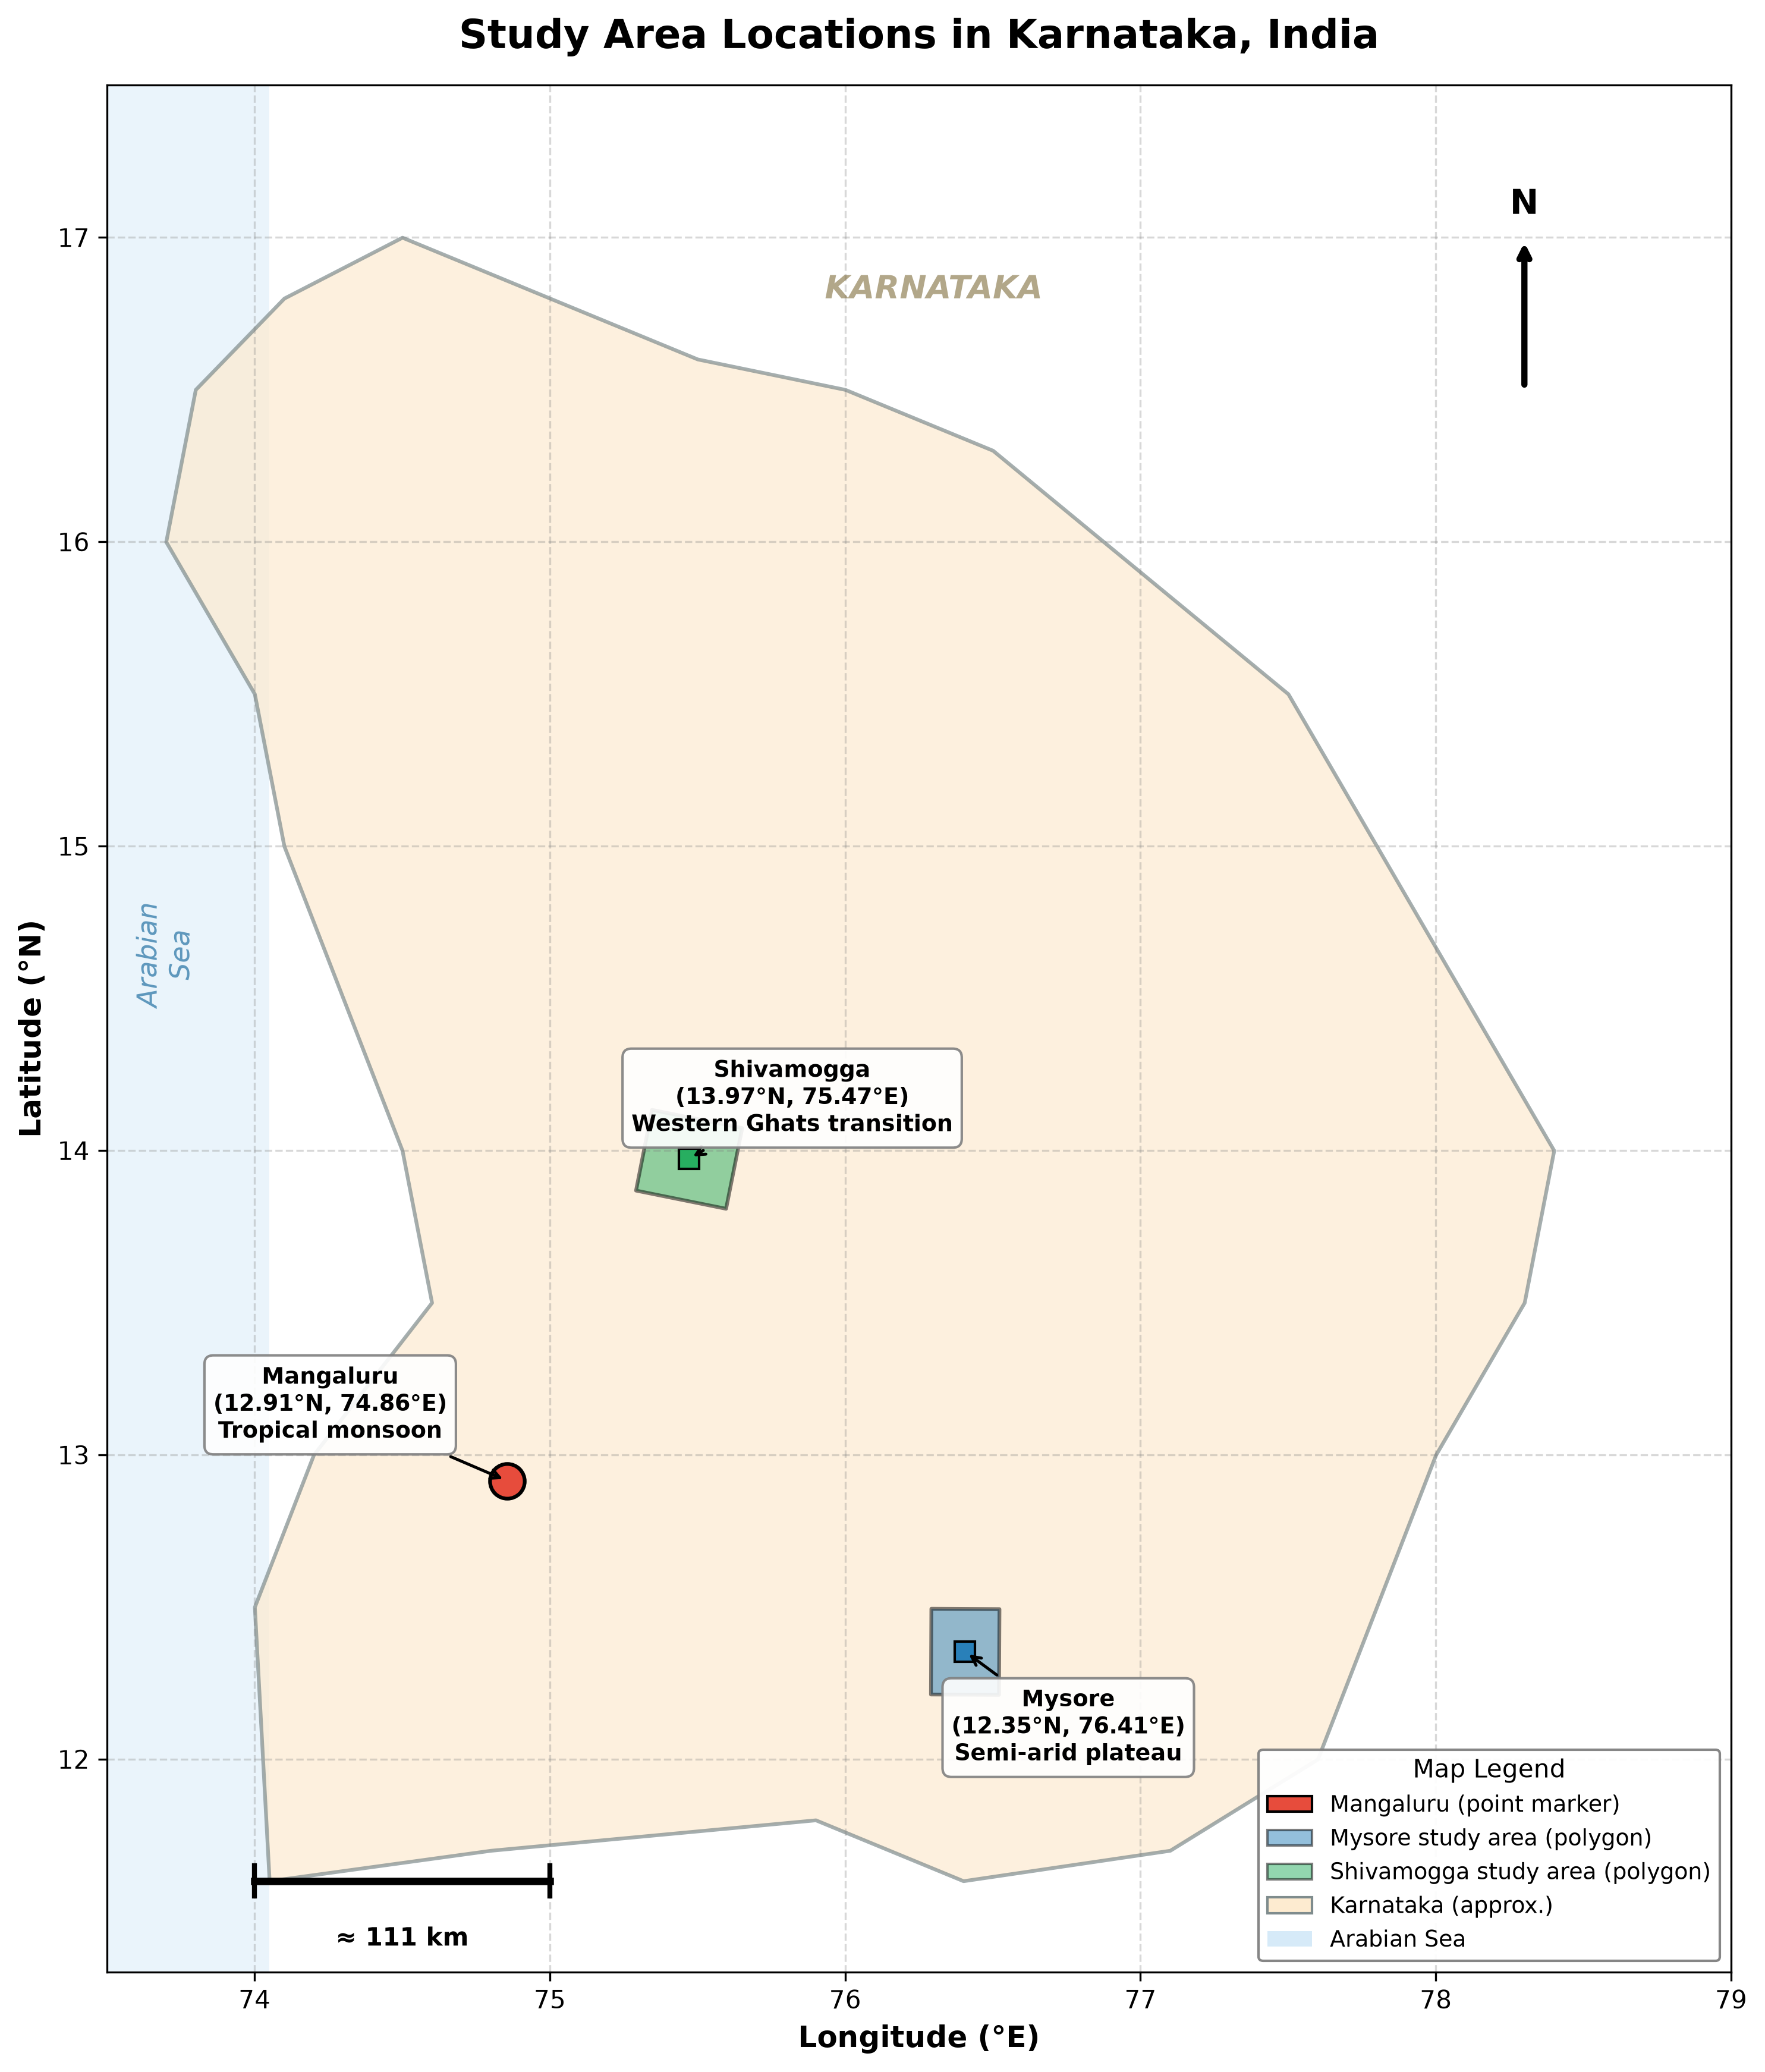
\includegraphics[width=0.88\textwidth]{figures/fig_study_area_map.png}
\caption{Geographical locations and shapefile boundaries of the three study areas in Karnataka, India: Mangaluru (coastal point location), Mysore (southern plateau polygon), and Shivamogga (Western Ghats transition polygon), highlighting regional climatic contrasts.}
\label{fig:study_area_map}
\end{figure}

\begin{table}[H]
\centering
\caption{Geographic and hydro-climatic characteristics of the three study areas}
\label{tab:study_sites}
\begin{tabular}{lcccc}
\toprule
\textbf{Study Site} & \textbf{Coordinates} & \textbf{Agro-Climatic Zone} & \textbf{Elevation} & \textbf{Ann. Rainfall} \\
\midrule
Mangaluru  & $12.9141^\circ$~N, $74.8560^\circ$~E & Coastal Lowland (\textit{Am}) & $\approx 20$~m  & $\approx 3,510$~mm \\
Mysore     & $12.3537^\circ$~N, $76.4054^\circ$~E & Southern Plateau (\textit{BSh})& $\approx 770$~m & $\approx 1,087$~mm \\
Shivamogga & $13.9719^\circ$~N, $75.4704^\circ$~E & Ghats Transition (\textit{Aw/Cwa}) & $\approx 640$~m & $\approx 1,162$~mm \\
\bottomrule
\end{tabular}
\end{table}

% ══════════════════════════════════════════════════════════════════════
%  CHAPTER 2 — CONCEPTS AND THEORY
% ══════════════════════════════════════════════════════════════════════

\section{Key Concepts and Theoretical Background}

\subsection{What Is Soil Moisture?}

Soil moisture, in the context of this project, refers to \textbf{volumetric water content} --- the fraction of a given volume of soil that is occupied by water. It is expressed in units of m\textsuperscript{3}/m\textsuperscript{3} (cubic metres of water per cubic metre of soil). A value of 0.30, for example, means that 30\% of the soil volume is water.

Soil moisture varies across depth. The surface layer (0--7~cm) responds rapidly to rainfall and evaporation, often changing substantially within a single day. Deeper layers (7--28~cm and 28--100~cm) act as reservoirs: water percolates downward over days to weeks, and these layers change more slowly. For agricultural decision-making, the deeper root-zone moisture is often more important than the surface value, because it determines how much water is actually accessible to crop roots.

\subsection{ERA5-Land Reanalysis}

ERA5-Land is a land-surface reanalysis dataset produced by the ECMWF. It combines:

\begin{itemize}
    \item Atmospheric forcing data from the ERA5 atmospheric reanalysis (temperature, humidity, wind, precipitation, radiation).
    \item A sophisticated land surface model (HTESSEL) that simulates infiltration, percolation, evapotranspiration, and runoff.
\end{itemize}

The result is a physically consistent estimate of soil moisture at multiple depths, updated hourly, with global coverage at approximately 9~km spatial resolution. We access this data through the Open-Meteo archive API, which provides it in a convenient format.

\textbf{Important caveat:} ERA5-Land values are \textit{modelled} estimates, not direct sensor measurements. They can differ from actual field conditions, particularly in regions with unusual soil types or land cover that the model does not represent well. In this project, ERA5-Land serves as both the training target and the primary validation reference.

\subsection{Machine Learning for Time-Series Forecasting}

\subsubsection{The Regression Problem}

At its core, soil moisture forecasting is a \textbf{supervised regression} problem. Given a set of input features $\mathbf{x}$ (such as yesterday's soil moisture, today's temperature, and today's rainfall), we want to learn a function $f$ such that:
\[
\hat{y} = f(\mathbf{x})
\]
where $\hat{y}$ is the predicted soil moisture for tomorrow. The function $f$ is learned from historical data where both the inputs and the true outputs are known.

\subsubsection{XGBoost: Extreme Gradient Boosting}

XGBoost (Extreme Gradient Boosting) is the primary machine learning algorithm used in this project. It belongs to the family of \textbf{ensemble methods} --- approaches that combine many simple models to produce a powerful overall prediction.

\paragraph{Decision Trees.} The building block of XGBoost is the \textit{decision tree}: a model that makes predictions by asking a series of yes/no questions about the input features. For example: ``Is yesterday's soil moisture above 0.15?'' $\rightarrow$ ``Is today's rainfall above 5~mm?'' Each path through the tree leads to a predicted value.

A single decision tree is easy to interpret but tends to be either too simple (underfitting) or too sensitive to the specific training data (overfitting).

\paragraph{Gradient Boosting.} Gradient boosting addresses this by building trees \textit{sequentially}. The first tree makes a rough prediction. The second tree is trained not on the original target values, but on the \textit{errors} (residuals) that the first tree made. The third tree corrects the remaining errors, and so on. Each new tree focuses on the mistakes that all previous trees collectively failed to fix. The final prediction is the sum of all trees' outputs:
\[
\hat{y} = \sum_{k=1}^{K} f_k(\mathbf{x})
\]
where $K$ is the total number of trees and each $f_k$ is a small decision tree.

\paragraph{Why XGBoost?} XGBoost adds several engineering refinements to this basic idea:
\begin{itemize}
    \item \textbf{Regularisation}: Penalties that prevent individual trees from becoming too complex, reducing overfitting.
    \item \textbf{Second-order optimisation}: Uses both the gradient and the curvature of the loss function for more efficient training.
    \item \textbf{Handling of missing values}: Natively handles gaps in input data.
    \item \textbf{Computational speed}: Highly optimised for fast parallel training.
\end{itemize}

In the context of soil moisture, XGBoost is well-suited because it can capture non-linear relationships (e.g., the highly asymmetric response of soil moisture to heavy rainfall versus dry spells) without requiring explicit physical equations.

\subsubsection{Recursive Multi-Step Forecasting}

To forecast more than one day ahead, we use a \textbf{recursive} (also called ``iterated'') strategy:

\begin{enumerate}
    \item The model predicts soil moisture for day $t+1$ using observed values at days $t$ and $t-1$.
    \item That prediction $\widehat{\text{SM}}_{t+1}$ is then fed back as an input to predict day $t+2$.
    \item The process repeats for up to 7 days.
\end{enumerate}

Mathematically, for each forecast step $k$:
\[
\widehat{\text{SM}}_{t+k} = f\!\left(\widehat{\text{SM}}_{t+k-1},\ \widehat{\text{SM}}_{t+k-2},\ \mathbf{W}_{t+k}\right)
\]
where $\mathbf{W}_{t+k}$ represents the weather variables (from a weather forecast) for day $t+k$, and SM values for $k \leq 2$ come from actual observations.

The key challenge with recursive forecasting is \textbf{error accumulation}: any error in the day-1 prediction becomes part of the input for day-2, potentially causing errors to compound. Robust models with regularisation (like XGBoost) mitigate this, but accuracy inevitably degrades with forecast horizon.

\subsection{Evaluation Metrics}

We use two standard metrics to evaluate model performance:

\paragraph{Coefficient of Determination ($R^2$).}
\[
R^2 = 1 - \frac{\sum_i (y_i - \hat{y}_i)^2}{\sum_i (y_i - \bar{y})^2}
\]
An $R^2$ of 1.0 means perfect predictions. An $R^2$ of 0.0 means the model is no better than always predicting the mean. Negative $R^2$ means worse than the mean --- the model is actively harmful.

\paragraph{Root Mean Squared Error (RMSE).}
\[
\text{RMSE} = \sqrt{\frac{1}{n}\sum_{i=1}^{n}(y_i - \hat{y}_i)^2}
\]
RMSE is in the same units as the target variable (m\textsuperscript{3}/m\textsuperscript{3}), making it directly interpretable. An RMSE of 0.03 means the model's predictions are, on average, about 0.03 m\textsuperscript{3}/m\textsuperscript{3} away from the truth.

\paragraph{Persistence Baseline.} A critical benchmark in time-series forecasting: the ``persistence'' model simply predicts that tomorrow's soil moisture will be the same as today's. Any useful model must beat persistence. This is a surprisingly strong baseline for slowly-varying quantities like soil moisture.

% ══════════════════════════════════════════════════════════════════════
%  CHAPTER 3 — DATA
% ══════════════════════════════════════════════════════════════════════

\section{Data Sources and Preparation}

\subsection{ERA5-Land Reanalysis Data}

The primary dataset is retrieved from the \textbf{Open-Meteo archive API}, which provides ERA5-Land variables for any specified location and date range. For all three study sites --- Mangaluru ($12.9141^\circ$~N, $74.8560^\circ$~E), Mysore ($12.3537^\circ$~N, $76.4054^\circ$~E), and Shivamogga ($13.9719^\circ$~N, $75.4704^\circ$~E) --- we obtained hourly data from \textbf{January 2023 to December 2025} (3 years; 1,096 complete daily timesteps per site), covering the identical temporal window to enable rigorous cross-site comparisons.

Hourly values are aggregated to daily resolution to produce the following feature set:

\begin{table}[H]
\centering
\caption{Daily features derived from ERA5-Land and ERA5 atmospheric data}
\label{tab:features}
\begin{tabular}{lll}
\toprule
\textbf{Variable} & \textbf{Description} & \textbf{Aggregation} \\
\midrule
\texttt{sm\_0\_7} & Surface soil moisture (0--7~cm) & Daily mean \\
\texttt{sm\_7\_28} & Intermediate root-zone (7--28~cm) & Daily mean \\
\texttt{sm\_28\_100} & Deep root-zone (28--100~cm) & Daily mean \\
\texttt{t\_mean}, \texttt{t\_max}, \texttt{t\_min} & 2-m air temperature & Mean / Max / Min \\
\texttt{t\_range} & Diurnal temperature range & $T_{\max} - T_{\min}$ \\
\texttt{rh\_mean}, \texttt{rh\_max}, \texttt{rh\_min} & Relative humidity & Mean / Max / Min \\
\texttt{pressure} & Surface atmospheric pressure & Daily mean \\
\texttt{wind\_mean}, \texttt{wind\_max} & 10-m wind speed & Mean / Max \\
\texttt{rain} & Total precipitation & Daily sum (mm) \\
\texttt{rain\_1d}, \texttt{rain\_2d} & Antecedent precipitation & Previous 1 and 2 days \\
\bottomrule
\end{tabular}
\end{table}

\subsection{Long-Memory Features}

A key extension beyond the reference paper is the inclusion of \textbf{long-memory features} that capture the slow hydrological response of deeper soil layers:

\begin{itemize}
    \item \texttt{rain\_7d}, \texttt{rain\_14d}, \texttt{rain\_30d}: Cumulative rainfall over the past 7, 14, and 30 days.
    \item \texttt{sm\_mean7}, \texttt{sm\_mean30}: Rolling average surface soil moisture over 7 and 30 days.
    \item \texttt{t\_mean7}: Rolling 7-day average temperature.
\end{itemize}

These features encode the ``memory'' of the soil system. For example, deep-layer moisture at 28--100~cm is largely insensitive to a single day's rain but responds strongly to whether the past month has been consistently wet or dry.

\subsection{ECMWF Archived Weather Forecasts}

For the surface forecasting model, we also retrieved \textbf{archived ECMWF IFS 0.25\textdegree\ weather forecasts} from the Open-Meteo Previous Runs API. These are the actual operational numerical weather predictions that were issued on each historical date, at lead times of 1 to 7 days.

This is a crucial distinction: instead of telling the model ``here is the weather that actually happened on day $t+k$'' (which is unrealistically perfect information), we use ``here is what the weather forecast \textit{predicted} would happen on day $t+k$, as issued $k$ days earlier''. This makes the model aware of the inherent noise and systematic biases in weather forecasts.

\subsection{Sentinel-1 and Sentinel-2 Satellite Data}

For the satellite feasibility study, we accessed data from the Copernicus programme via Google Earth Engine:

\begin{itemize}
    \item \textbf{Sentinel-1 SAR} (Synthetic Aperture Radar): C-band radar backscatter in VV and VH polarisations. Radar signals interact with soil dielectric properties, which are strongly influenced by water content. Unlike optical sensors, SAR can image through clouds --- critical during the monsoon.
    
    \item \textbf{Sentinel-2 MSI}: Multispectral optical imagery used to derive the Normalised Difference Vegetation Index (NDVI), which characterises vegetation density. NDVI is relevant because vegetation cover affects the radar--soil moisture relationship.
\end{itemize}

Data was extracted for a 150~m buffer around the study point, yielding approximately 75 usable Sentinel-1 scenes and a smaller number of cloud-free Sentinel-2 observations across 2023--2025.

\subsection{Data Splitting Strategy}

A critical methodological choice in time-series machine learning is how to split data into training and test sets.

\paragraph{Random splitting (the paper's approach):} Randomly assigning days to training or test sets. This is standard in many ML applications but is \textbf{problematic for time series}: because adjacent days are very similar, a random split allows the model to ``see'' nearly identical conditions in training that appear in the test set. This leads to overly optimistic performance estimates.

\paragraph{Chronological splitting (our primary approach):} All data before a cutoff date is used for training; all data after is used for testing. This simulates the real-world scenario where we must predict the future from the past, and produces honest, conservative performance estimates.

In this project:
\begin{itemize}
    \item \textbf{Training period}: January 2023 -- mid-2025 (approximately 80\% of the data).
    \item \textbf{Test period}: Mid-2025 -- December 2025 for deep-layer models; January -- October 2026 (out-of-sample) for the surface forecast model.
\end{itemize}

% ══════════════════════════════════════════════════════════════════════
%  CHAPTER 4 — METHODOLOGY
% ══════════════════════════════════════════════════════════════════════

\section{Methodology}

The overall system consists of three interconnected components (Figure~\ref{fig:pipeline}): a surface soil moisture forecaster, a progressive deep-layer estimator, and a satellite feasibility module.

\begin{figure}[H]
\centering
\fbox{\parbox{0.9\textwidth}{\centering
\textbf{System Pipeline Overview}\\[0.5cm]
\textit{Weather Data + Past Soil Moisture}\\
$\downarrow$\\
\textbf{Surface Forecaster} (XGBoost, recursive, 7-day horizon)\\
$\downarrow$ \textit{Surface SM estimate}\\
\textbf{Deep Layer 1 Model} (Surface SM + Weather $\rightarrow$ 7--28~cm)\\
$\downarrow$ \textit{Estimated 7--28~cm}\\
\textbf{Deep Layer 2 Model} (Surface + Layer 1 estimate + Weather $\rightarrow$ 28--100~cm)\\
$\downarrow$\\
\textit{Complete soil moisture profile: 0--7, 7--28, 28--100~cm}
}}
\caption{Overview of the modelling pipeline. The surface forecast feeds into the deep-layer estimators in a progressive chain.}
\label{fig:pipeline}
\end{figure}

\subsection{Component 1: Surface Soil Moisture Forecasting (0--7~cm)}

\subsubsection{Model Architecture}

The surface forecaster is an XGBoost regressor that predicts today's surface soil moisture from:
\begin{itemize}
    \item \textbf{Autoregressive inputs}: Surface moisture from the previous two days (SM$_{t-1}$ and SM$_{t-2}$).
    \item \textbf{Weather inputs}: Maximum temperature, minimum temperature, mean relative humidity, and total rainfall for the target day.
    \item \textbf{Lead time}: An integer (1 to 7) indicating how far into the future the prediction is.
\end{itemize}

The inclusion of lead time as a feature is an innovation of this project. It allows a single model to learn that longer-range forecasts should rely more on autoregressive momentum and less on weather inputs (since weather forecasts become noisier at longer horizons).

\subsubsection{Training on Real Weather Forecasts}

The reference paper trains the surface model using \textit{observed} (ERA5 reanalysis) weather as the input, even for multi-day-ahead predictions. This is equivalent to giving the model a perfect crystal ball for future weather, which is unrealistic.

We instead train the model on \textbf{archived ECMWF operational forecasts} at matching lead times. For a training example targeting lead $k$:
\begin{itemize}
    \item The soil moisture lags come from ERA5-Land observations.
    \item The weather inputs come from the ECMWF forecast that was issued $k$ days before the target date.
\end{itemize}

This means the model learns to work with the imperfect, noisy weather forecasts it will actually receive in operation, rather than being surprised by forecast errors at deployment time.

\subsubsection{Hyperparameters}

The model uses 400 boosting rounds, a maximum tree depth of 3, and a learning rate of 0.05. These were selected through 5-fold time-series cross-validation on the training data.

\subsection{Component 2: Progressive Deep-Layer Estimation}

\subsubsection{Rationale}

Surface soil moisture responds quickly to atmospheric forcing (rain, evaporation). Deeper layers respond more slowly as water percolates downward. Rather than directly predicting deep-layer moisture from weather alone, we use a \textbf{progressive chain}:

\begin{enumerate}
    \item \textbf{Model 1}: Predicts 7--28~cm moisture from surface moisture (0--7~cm) plus all weather features and long-memory features.
    \item \textbf{Model 2}: Predicts 28--100~cm moisture from \textit{the output of Model 1} (estimated 7--28~cm) plus surface moisture and the same weather features.
\end{enumerate}

This chaining mirrors the physical process of vertical water movement: surface conditions drive intermediate-depth moisture, which in turn drives deep-layer moisture.

\subsubsection{Feature Set}

Each deep-layer model receives 20 input features:

\begin{itemize}
    \item Surface soil moisture (\texttt{sm\_0\_7}).
    \item For Model 2: estimated 7--28~cm moisture (\texttt{sm\_7\_28}).
    \item 13 meteorological variables (temperature statistics, humidity, pressure, wind, rainfall and antecedent rainfall).
    \item 6 long-memory features (rolling precipitation sums, rolling soil moisture and temperature means).
\end{itemize}

\subsubsection{Model Selection}

Three algorithms were compared: Linear Regression (LR), Random Forest (RF), and XGBoost (XGB). Each was tuned via grid search with 5-fold time-series cross-validation. XGBoost with long-memory features consistently achieved the best results and was selected for deployment.

\subsection{Component 3: Satellite Remote Sensing Feasibility}

\subsubsection{Sentinel-1 Radar and Soil Moisture}

Synthetic Aperture Radar (SAR) at C-band frequency is sensitive to soil dielectric properties, which are primarily governed by water content. The Sentinel-1 satellite provides VV (co-polarised) and VH (cross-polarised) backscatter coefficients.

However, backscatter is also affected by surface roughness, vegetation structure, and incidence angle. At a tropical site like Mangaluru, the strong seasonal cycle of vegetation growth (dense during monsoon, sparse in summer) creates a confounding signal that can mask the moisture response.

\subsubsection{Anomaly-Based Retrieval}

To isolate the moisture signal from the seasonal cycle, we employ an \textbf{anomaly-based approach}:
\begin{enumerate}
    \item Compute the monthly climatological mean of both backscatter (VV) and soil moisture.
    \item Subtract the climatology to obtain anomalies: how much wetter or drier than normal is this particular day?
    \item Use a linear regression to predict the soil moisture anomaly from the backscatter anomaly.
    \item Add the climatological soil moisture back to obtain the final estimate.
\end{enumerate}

This approach is evaluated using leave-one-year-out cross-validation across 2023--2025.

% ══════════════════════════════════════════════════════════════════════
%  CHAPTER 5 — RESULTS
% ══════════════════════════════════════════════════════════════════════

\section{Results and Analysis}

\subsection{Surface Forecast Performance}

\subsubsection{Out-of-Sample Test on 2026}

The surface forecast model was evaluated over 276 independent forecast origins spanning January to October 2026 --- a period the model had never seen during training (the model was trained on 2024--2025 data). Table~\ref{tab:forecast_r2} shows $R^2$ scores and Table~\ref{tab:forecast_rmse} shows RMSE values.

\begin{table}[H]
\centering
\caption{Surface forecast $R^2$ by forecast horizon (276 origins, Jan--Oct 2026)}
\label{tab:forecast_r2}
\begin{tabular}{cccc}
\toprule
\textbf{Day} & \textbf{Persistence} & \textbf{Trained on ERA5} & \textbf{Trained on Forecasts} \\
\midrule
1 & 0.9274 & 0.9228 & \textbf{0.9496} \\
2 & 0.8458 & 0.8437 & \textbf{0.9014} \\
3 & 0.7776 & 0.7745 & \textbf{0.8755} \\
4 & 0.7149 & 0.7166 & \textbf{0.8369} \\
5 & 0.6683 & 0.6493 & \textbf{0.7952} \\
6 & 0.6369 & 0.6101 & \textbf{0.7487} \\
7 & 0.5981 & 0.5860 & \textbf{0.7324} \\
\bottomrule
\end{tabular}
\end{table}

\begin{table}[H]
\centering
\caption{Surface forecast RMSE (m\textsuperscript{3}/m\textsuperscript{3}) by forecast horizon}
\label{tab:forecast_rmse}
\begin{tabular}{cccc}
\toprule
\textbf{Day} & \textbf{Persistence} & \textbf{Trained on ERA5} & \textbf{Trained on Forecasts} \\
\midrule
1 & 0.0327 & 0.0337 & \textbf{0.0272} \\
2 & 0.0476 & 0.0479 & \textbf{0.0380} \\
3 & 0.0571 & 0.0575 & \textbf{0.0427} \\
4 & 0.0646 & 0.0644 & \textbf{0.0489} \\
5 & 0.0697 & 0.0717 & \textbf{0.0548} \\
6 & 0.0729 & 0.0755 & \textbf{0.0606} \\
7 & 0.0766 & 0.0778 & \textbf{0.0625} \\
\bottomrule
\end{tabular}
\end{table}

\textbf{Key observations:}
\begin{itemize}
    \item The model trained on real ECMWF forecasts \textbf{significantly outperforms} both persistence and the ERA5-trained model at every horizon.
    \item The ERA5-trained model actually performs \textit{worse} than persistence at some horizons. This is because it was trained with perfect weather inputs but tested with imperfect forecasts --- a form of train/test distribution mismatch.
    \item Even at day~7, the forecast-trained model maintains $R^2 = 0.73$ and RMSE $= 0.063$~m\textsuperscript{3}/m\textsuperscript{3}, demonstrating useful skill.
\end{itemize}

\subsubsection{Comparison with Oracle Weather}

An ``oracle'' model that uses perfect (ERA5) future weather provides an upper bound on achievable skill. Table~\ref{tab:oracle} compares oracle, real-forecast, and persistence models from the 2025 test period.

\begin{table}[H]
\centering
\caption{7-day forecast $R^2$: oracle (perfect weather) vs real ECMWF forecasts vs persistence (2025 test)}
\label{tab:oracle}
\begin{tabular}{cccc}
\toprule
\textbf{Day} & \textbf{Oracle (ERA5)} & \textbf{Real Forecast} & \textbf{Persistence} \\
\midrule
1 & 0.9753 & 0.9626 & 0.9380 \\
3 & 0.9553 & 0.9029 & 0.7775 \\
5 & 0.9421 & 0.8513 & 0.6558 \\
7 & 0.9377 & 0.8179 & 0.5752 \\
\bottomrule
\end{tabular}
\end{table}

The gap between oracle and real-forecast performance quantifies the cost of weather forecast errors. At day~1, this gap is small (0.013 in $R^2$); by day~7, it grows to 0.12 --- indicating that improved weather forecasts would directly improve soil moisture predictions.

\subsubsection{Robustness to Weather Forecast Noise}

To understand how the model degrades under different levels of weather forecast quality, we tested with synthetically degraded weather inputs:

\begin{table}[H]
\centering
\caption{Forecast $R^2$ under varying weather input quality (day~7)}
\label{tab:robustness}
\begin{tabular}{lc}
\toprule
\textbf{Weather Scenario} & \textbf{Day-7 $R^2$} \\
\midrule
Oracle (perfect weather) & 0.9377 \\
Mild noise ($\sigma_T = 1$\textdegree C, $\sigma_{\text{rain}} = 50\%$) & 0.8954 \\
Heavy noise ($\sigma_T = 2$\textdegree C, $\sigma_{\text{rain}} = 100\%$) & 0.7944 \\
No forecast (climatological mean weather) & 0.4386 \\
Persistence baseline & 0.5752 \\
\bottomrule
\end{tabular}
\end{table}

Even under heavy noise, the model ($R^2 = 0.79$) substantially outperforms persistence (0.58). However, replacing weather forecasts entirely with climatological averages drops performance below persistence, confirming that weather forecast information is essential.

\subsection{Deep-Layer Estimation Performance}

\subsubsection{Effect of Long-Memory Features}

Table~\ref{tab:deep_layer} compares the deep-layer models with and without the long-memory features, on the chronological test set (June--December 2025).

\begin{table}[H]
\centering
\caption{Deep-layer estimation performance: paper-style features vs.\ long-memory features (XGBoost, chronological test)}
\label{tab:deep_layer}
\begin{tabular}{llcc}
\toprule
\textbf{Layer} & \textbf{Feature Set} & \textbf{$R^2$} & \textbf{RMSE} \\
\midrule
\multirow{2}{*}{7--28~cm} & Base (paper-style) & 0.9253 & 0.0264 \\
                          & Base + long memory  & \textbf{0.9785} & \textbf{0.0142} \\
\midrule
\multirow{2}{*}{28--100~cm} & Base (paper-style) & 0.3524 & 0.0629 \\
                            & Base + long memory  & \textbf{0.7439} & \textbf{0.0395} \\
\bottomrule
\end{tabular}
\end{table}

\textbf{Key observations:}
\begin{itemize}
    \item Long-memory features dramatically improve deep-layer estimation, particularly for the 28--100~cm layer where $R^2$ more than doubles from 0.35 to 0.74.
    \item This makes physical sense: deeper soil responds to cumulative precipitation over weeks, not individual daily events.
    \item The 7--28~cm layer is well-estimated regardless, with $R^2 > 0.97$ when long-memory features are included.
\end{itemize}

\subsubsection{Random vs.\ Chronological Split Comparison}

To quantify the data-leakage problem, Table~\ref{tab:split} compares performance under random and chronological splitting.

\begin{table}[H]
\centering
\caption{Deep-layer $R^2$ with weather features: random split vs.\ chronological split}
\label{tab:split}
\begin{tabular}{lccc}
\toprule
\textbf{Layer} & \textbf{Model} & \textbf{Random Split} & \textbf{Chronological Split} \\
\midrule
\multirow{3}{*}{7--28~cm} & LR  & 0.935 & 0.920 \\
                          & RF  & 0.967 & 0.933 \\
                          & XGB & 0.966 & 0.935 \\
\midrule
\multirow{3}{*}{28--100~cm} & LR  & 0.615 & 0.464 \\
                            & RF  & 0.710 & 0.396 \\
                            & XGB & 0.700 & 0.355 \\
\bottomrule
\end{tabular}
\end{table}

The random split consistently overstates performance, especially for the 28--100~cm layer. For RF, the random-split $R^2$ of 0.71 drops to 0.40 under chronological splitting --- a stark reminder that random splits can give a misleading picture of real-world model performance for time-series problems.

\subsubsection{2026 Out-of-Sample Backtest}

The deployed deep-layer models were tested on all of 2026 (data they were never trained on). Table~\ref{tab:deep2026} summarises the results.

\begin{table}[H]
\centering
\caption{Deep-layer estimation on 2026 data (models trained through 2025)}
\label{tab:deep2026}
\begin{tabular}{lcccc}
\toprule
\textbf{Layer} & \textbf{n (days)} & \textbf{$R^2$} & \textbf{RMSE} & \textbf{Bias} \\
\midrule
7--28~cm   & 296 & 0.9746 & 0.0173 & $-0.0037$ \\
28--100~cm & 296 & 0.8041 & 0.0398 & $+0.0105$ \\
\bottomrule
\end{tabular}
\end{table}

The 7--28~cm model generalises extremely well with an $R^2$ of 0.97 on unseen data. The 28--100~cm model shows a slight high bias (+0.01) but maintains strong overall performance. Performance is best during the monsoon months (June--September) and degrades somewhat in the dry early months of the year.

\subsection{Seasonal Performance Patterns}

The 7-day forecast was evaluated separately for dry/pre-monsoon (January--May) and monsoon (June--September) seasons.

\begin{table}[H]
\centering
\caption{Surface forecast RMSE by season (2026 backtest, real forecasts)}
\label{tab:seasonal}
\begin{tabular}{lccc}
\toprule
\textbf{Season} & \textbf{Day~1 RMSE} & \textbf{Day~3 RMSE} & \textbf{Day~7 RMSE} \\
\midrule
Dry/pre-monsoon (Jan--May) & 0.0338 & 0.0537 & 0.0737 \\
Monsoon (Jun--Sep)         & 0.0335 & 0.0619 & 0.0827 \\
\bottomrule
\end{tabular}
\end{table}

Monsoon forecasts are slightly less accurate at longer horizons due to the greater variability of daily rainfall, but the model remains skillful in both seasons.

\subsection{Satellite Feasibility Results}

The satellite module evaluated whether Sentinel-1 radar backscatter can independently estimate surface soil moisture using leave-one-year-out cross-validation across 75 scenes.

\begin{table}[H]
\centering
\caption{Sentinel-1 feasibility: $R^2$ vs ERA5 surface moisture (leave-one-year-out)}
\label{tab:satellite}
\begin{tabular}{lc}
\toprule
\textbf{Model} & \textbf{$R^2$} \\
\midrule
Month climatology (no radar) & 0.725 \\
Linear Regression: VV only & 0.628 \\
Linear Regression: VV + VH & 0.613 \\
Random Forest: VV, VH, RVI & 0.645 \\
Random Forest: VV, VH, RVI + month & 0.698 \\
Climatology + VV anomaly (our approach) & \textbf{0.811} \\
\bottomrule
\end{tabular}
\end{table}

\textbf{Key observations:}
\begin{itemize}
    \item Raw radar-based models (LR, RF) perform \textit{worse} than simple monthly climatology. This is because at Mangaluru, the annual vegetation cycle dominates the radar signal, and a naive model confuses vegetation changes with moisture changes.
    \item The anomaly-based approach, which subtracts the seasonal cycle from both radar and moisture, achieves $R^2 = 0.81$ --- demonstrating that Sentinel-1 provides genuine day-to-day information beyond climatology.
    \item This suggests that radar data could serve as an independent validation source, but further work is needed before it could replace reanalysis data.
\end{itemize}

% ══════════════════════════════════════════════════════════════════════
%  CHAPTER 6 — OPERATIONAL DASHBOARD
% ══════════════════════════════════════════════════════════════════════

\section{Operational Dashboard}

A live Streamlit web application was developed to demonstrate the models in an operational setting. The application performs the following steps each time it is loaded:

\begin{enumerate}
    \item \textbf{Fetches the latest ERA5-Land observations} from the Open-Meteo archive. Due to processing delays, the most recent ERA5 day is typically 2--5 days behind the current date.
    
    \item \textbf{Fetches the latest weather forecast} from the Open-Meteo forecast API (ECMWF-based) for the next 7+ days.
    
    \item \textbf{Bridges the latency gap}: For the days between the last ERA5 observation and today, the model uses forecast weather to recursively predict surface moisture.
    
    \item \textbf{Extends the forecast} up to 7 days into the future from the current date.
    
    \item \textbf{Chains through the deep-layer models} to produce estimates of 7--28~cm and 28--100~cm moisture for all dates.
    
    \item \textbf{Displays the results} in an interactive dashboard with:
    \begin{itemize}
        \item Time-series plots of observed and forecasted surface moisture, with $\pm 1$~RMSE uncertainty bands.
        \item Side-by-side plots of deep-layer estimates vs.\ ERA5 observations.
        \item Frozen evaluation tables from the offline experiments.
        \item Methodology notes and limitations.
    \end{itemize}
\end{enumerate}

The dashboard prominently displays warnings that the system is a research prototype and that values are modelled estimates, not sensor measurements.

% ══════════════════════════════════════════════════════════════════════
%  CHAPTER 7 — MULTI-SITE COMPARATIVE ANALYSIS
% ══════════════════════════════════════════════════════════════════════

\section{Multi-Site Comparative Analysis}

To rigorously assess the generalisability of the machine learning framework, the entire empirical workflow was executed independently for each of the three study regions: \textbf{Mangaluru} (coastal tropical monsoon), \textbf{Mysore} (inland rain-shadow plateau), and \textbf{Shivamogga} (Western Ghats ecological transition zone). This section evaluates cross-regional model performance, hydrological responses, and climatic sensitivities.

\subsection{Cross-Site Surface Forecast Performance}

Table~\ref{tab:cross_forecast} and Figure~\ref{fig:fig6_forecast} compare the 7-day recursive surface soil moisture forecasting skill across all three sites using the identical XGBoost architecture.

\begin{table}[H]
\centering
\caption{Cross-site surface soil moisture (0--7~cm) forecasting performance ($R^2$ and RMSE in m$^3$/m$^3$)}
\label{tab:cross_forecast}
\begin{tabular}{lcccccc}
\toprule
\multirow{2}{*}{\textbf{Lead Day}} & \multicolumn{2}{c}{\textbf{Mangaluru}} & \multicolumn{2}{c}{\textbf{Mysore}} & \multicolumn{2}{c}{\textbf{Shivamogga}} \\
\cmidrule(lr){2-3} \cmidrule(lr){4-5} \cmidrule(lr){6-7}
& \textbf{$R^2$} & \textbf{RMSE} & \textbf{$R^2$} & \textbf{RMSE} & \textbf{$R^2$} & \textbf{RMSE} \\
\midrule
Day 1 & 0.9753 & 0.0182 & 0.9529 & 0.0174 & 0.9765 & 0.0134 \\
Day 2 & 0.9632 & 0.0222 & 0.9010 & 0.0252 & 0.9469 & 0.0203 \\
Day 3 & 0.9553 & 0.0245 & 0.8590 & 0.0300 & 0.9197 & 0.0251 \\
Day 4 & 0.9479 & 0.0265 & 0.8236 & 0.0334 & 0.8994 & 0.0282 \\
Day 5 & 0.9421 & 0.0279 & 0.7939 & 0.0360 & 0.8846 & 0.0304 \\
Day 6 & 0.9389 & 0.0287 & 0.7651 & 0.0382 & 0.8712 & 0.0323 \\
Day 7 & 0.9377 & 0.0294 & 0.7415 & 0.0400 & 0.8615 & 0.0336 \\
\midrule
\textit{Persist. (Day 1)} & \textit{0.9380} & \textit{0.0288} & \textit{0.9196} & \textit{0.0228} & \textit{0.9605} & \textit{0.0174} \\
\textit{Persist. (Day 7)} & \textit{0.5752} & \textit{0.0898} & \textit{0.2214} & \textit{0.0694} & \textit{0.7175} & \textit{0.0481} \\
\bottomrule
\end{tabular}
\end{table}

\paragraph{Key Insights on Surface Forecasting:}
\begin{itemize}
    \item \textbf{Universally Superior to Persistence:} Across all three distinct climatic regimes, the recursive XGBoost forecaster decisively outperforms the persistence benchmark at every lead horizon.
    \item \textbf{Extreme Persistence Failure in Semi-Arid Climates:} In Mysore, persistence rapidly degrades to $R^2 = 0.2214$ by Day 7 due to high solar radiation, strong convective drying, and sporadic flash rainfall events. The XGBoost model, however, maintains $R^2 = 0.7415$ (RMSE $= 0.0400$~m$^3$/m$^3$), demonstrating that meteorological coupling is exceptionally vital in semi-arid zones.
    \item \textbf{Transition Zone Stability:} Shivamogga displays high predictability ($R^2 = 0.9765$ at Day 1; $R^2 = 0.8615$ at Day 7) with the lowest absolute RMSE across all sites ($0.0134$ to $0.0336$~m$^3$/m$^3$).
\end{itemize}

\subsection{Cross-Site Deep-Layer Profile Estimation}

Table~\ref{tab:cross_deep} and Figure~\ref{fig:fig7_deep} present comparative evaluation metrics for the progressive chained deep-layer estimations (7--28~cm and 28--100~cm) across the three regions, isolating the effect of long-memory features.

\begin{table}[H]
\centering
\caption{Cross-site deep-layer estimation performance (XGBoost under chronological split)}
\label{tab:cross_deep}
\begin{tabular}{llcccc}
\toprule
\textbf{Site} & \textbf{Feature Set} & \multicolumn{2}{c}{\textbf{7--28 cm}} & \multicolumn{2}{c}{\textbf{28--100 cm}} \\
\cmidrule(lr){3-4} \cmidrule(lr){5-6}
& & \textbf{$R^2$} & \textbf{RMSE} & \textbf{$R^2$} & \textbf{RMSE} \\
\midrule
\multirow{2}{*}{\textbf{Mangaluru}}  & Base (paper-style) & 0.9253 & 0.0264 & 0.3524 & 0.0629 \\
                                      & Base + Long Memory & \textbf{0.9785} & \textbf{0.0142} & \textbf{0.7439} & \textbf{0.0395} \\
\midrule
\multirow{2}{*}{\textbf{Mysore}}     & Base (paper-style) & 0.8577 & 0.0263 & $-1.3790$ & 0.0588 \\
                                      & Base + Long Memory & \textbf{0.8655}\textsuperscript{*} & \textbf{0.0256} & $-1.0242$\textsuperscript{*} & \textbf{0.0543} \\
\midrule
\multirow{2}{*}{\textbf{Shivamogga}} & Base (paper-style) & 0.8872 & 0.0245 & 0.1991 & 0.0587 \\
                                      & Base + Long Memory & \textbf{0.9440} & \textbf{0.0173} & \textbf{0.4771} & \textbf{0.0475} \\
\bottomrule
\multicolumn{6}{l}{\footnotesize \textsuperscript{*}Random Forest achieved optimal performance on Mysore's deep layers.}
\end{tabular}
\end{table}

\paragraph{Hydrological Profile Mechanisms:}
\begin{itemize}
    \item \textbf{Intermediate Root-Zone (7--28~cm):} All three sites exhibit outstanding intermediate-layer estimation accuracy ($R^2 = 0.87$ to $0.98$; RMSE $< 0.026$~m$^3$/m$^3$). Chaining surface predictions downward captures intermediate soil percolation reliably across soil types.
    \item \textbf{Deep Layer (28--100~cm) and Rainfall Thresholds:} In Mangaluru and Shivamogga, where massive seasonal rainfall drives sustained downward moisture percolation, incorporating long-memory rolling averages ($7$ to $30$-day sums) doubles or triples explanatory power ($R^2$ jumps from $0.35 \rightarrow 0.74$ in Mangaluru, and $0.20 \rightarrow 0.48$ in Shivamogga).
    \item \textbf{The Rain-Shadow Semi-Arid Challenge (Mysore):} In Mysore, the deep root zone (28--100~cm) exhibits very low seasonal dynamic range ($0.13$ to $0.24$~m$^3$/m$^3$) because precipitation events rarely exceed the moisture deficit of the upper 28~cm profile. Under chronological testing, small deviations yield negative $R^2$, although absolute RMSE remains low ($\approx 0.054$~m$^3$/m$^3$), highlighting that deep-profile ML transferability depends intrinsically on whether surface forcing penetrates past the root barrier.
\end{itemize}

\subsection{Cross-Site Climatological Regimes and Water Balance}

Figure~\ref{fig:fig8_climatology} illustrates the 3-year daily and monthly climatologies for all three sites, illuminating the physical drivers behind the statistical metrics:

\begin{itemize}
    \item \textbf{Precipitation Volumes:} Mangaluru receives an extraordinary annual average of $3,509.9$~mm, predominantly delivered in massive monsoonal bursts ($>120$~mm/day). In contrast, Mysore receives $1,087.0$~mm and Shivamogga receives $1,161.6$~mm, characterised by intermittent convective pulses.
    \item \textbf{Layer Coupling Velocity:} In coastal Mangaluru, soil moisture at all three depths moves in lockstep during the monsoon peak, followed by steep exponential decay. In Mysore and Shivamogga, deep moisture experiences buffered attenuation, exhibiting substantial phase lags of 2 to 4 weeks relative to surface events.
\end{itemize}

% ══════════════════════════════════════════════════════════════════════
%  CHAPTER 8 — FIGURES
% ══════════════════════════════════════════════════════════════════════

\section{Figures}

This section presents the comprehensive suite of evaluation and comparative figures generated by the project.

\begin{figure}[H]
\centering
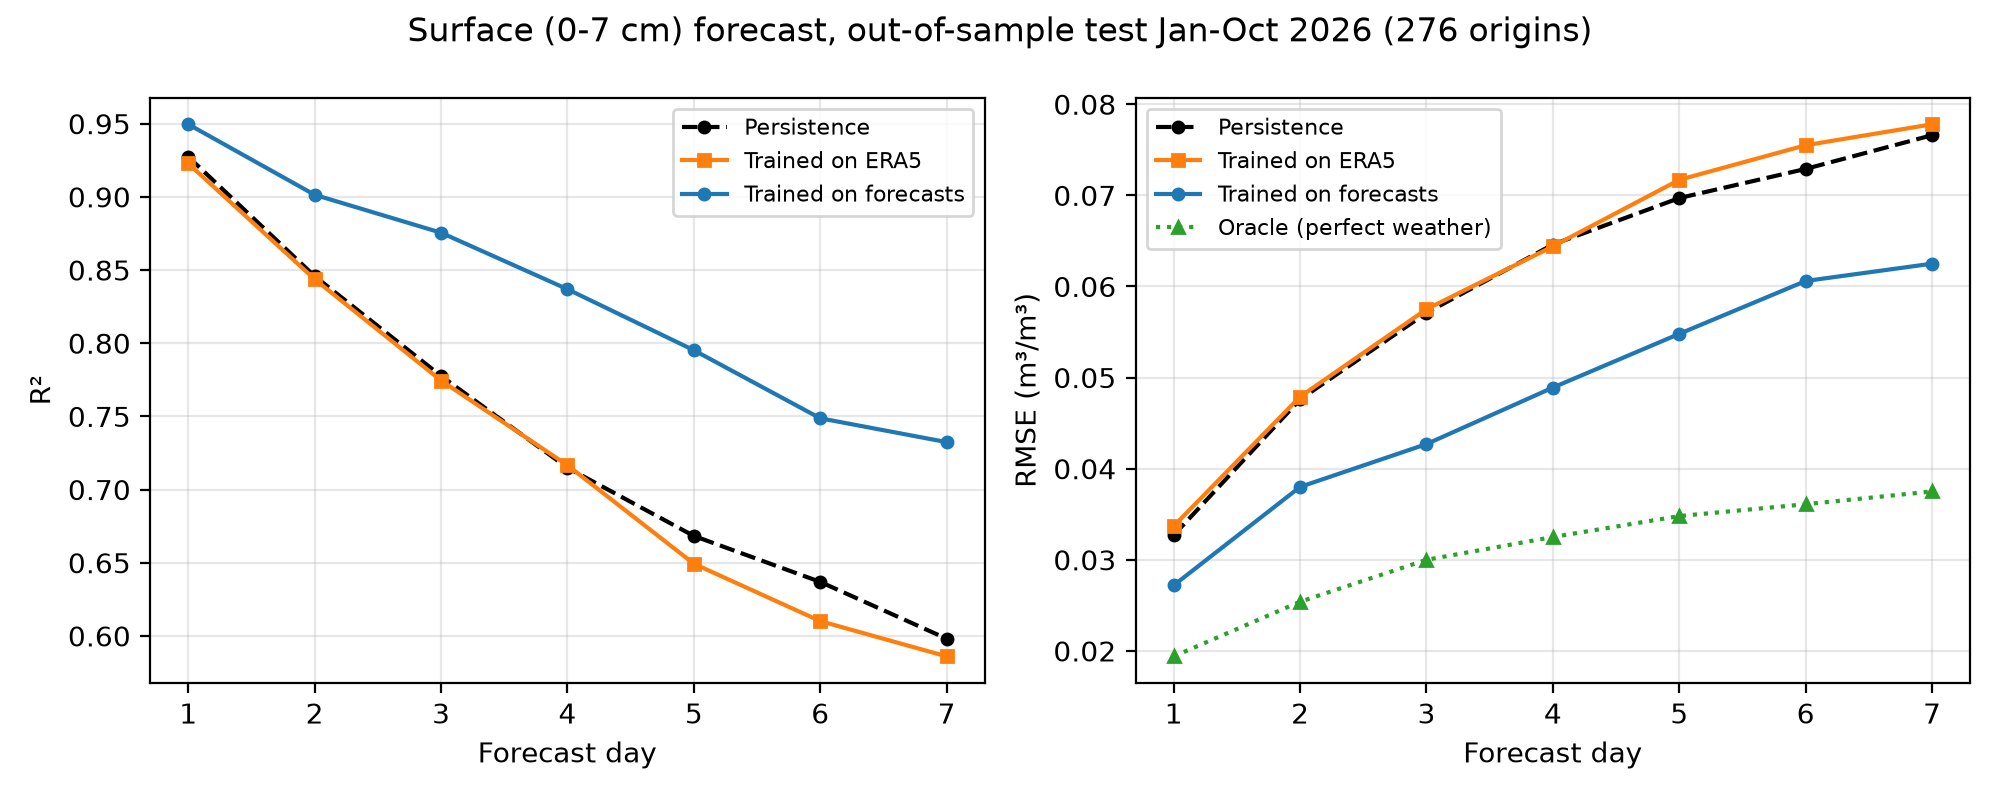
\includegraphics[width=0.95\textwidth]{figures/fig1_forecast_horizon.png}
\caption{Surface (0--7~cm) forecast performance by horizon for Mangaluru. Left: $R^2$. Right: RMSE. The model trained on archived ECMWF forecasts (blue) outperforms both persistence (black dashed) and the model trained on ERA5 weather (orange) at all lead times. The oracle line (green, right panel) shows the upper bound with perfect future weather.}
\label{fig:fig1}
\end{figure}

\begin{figure}[H]
\centering
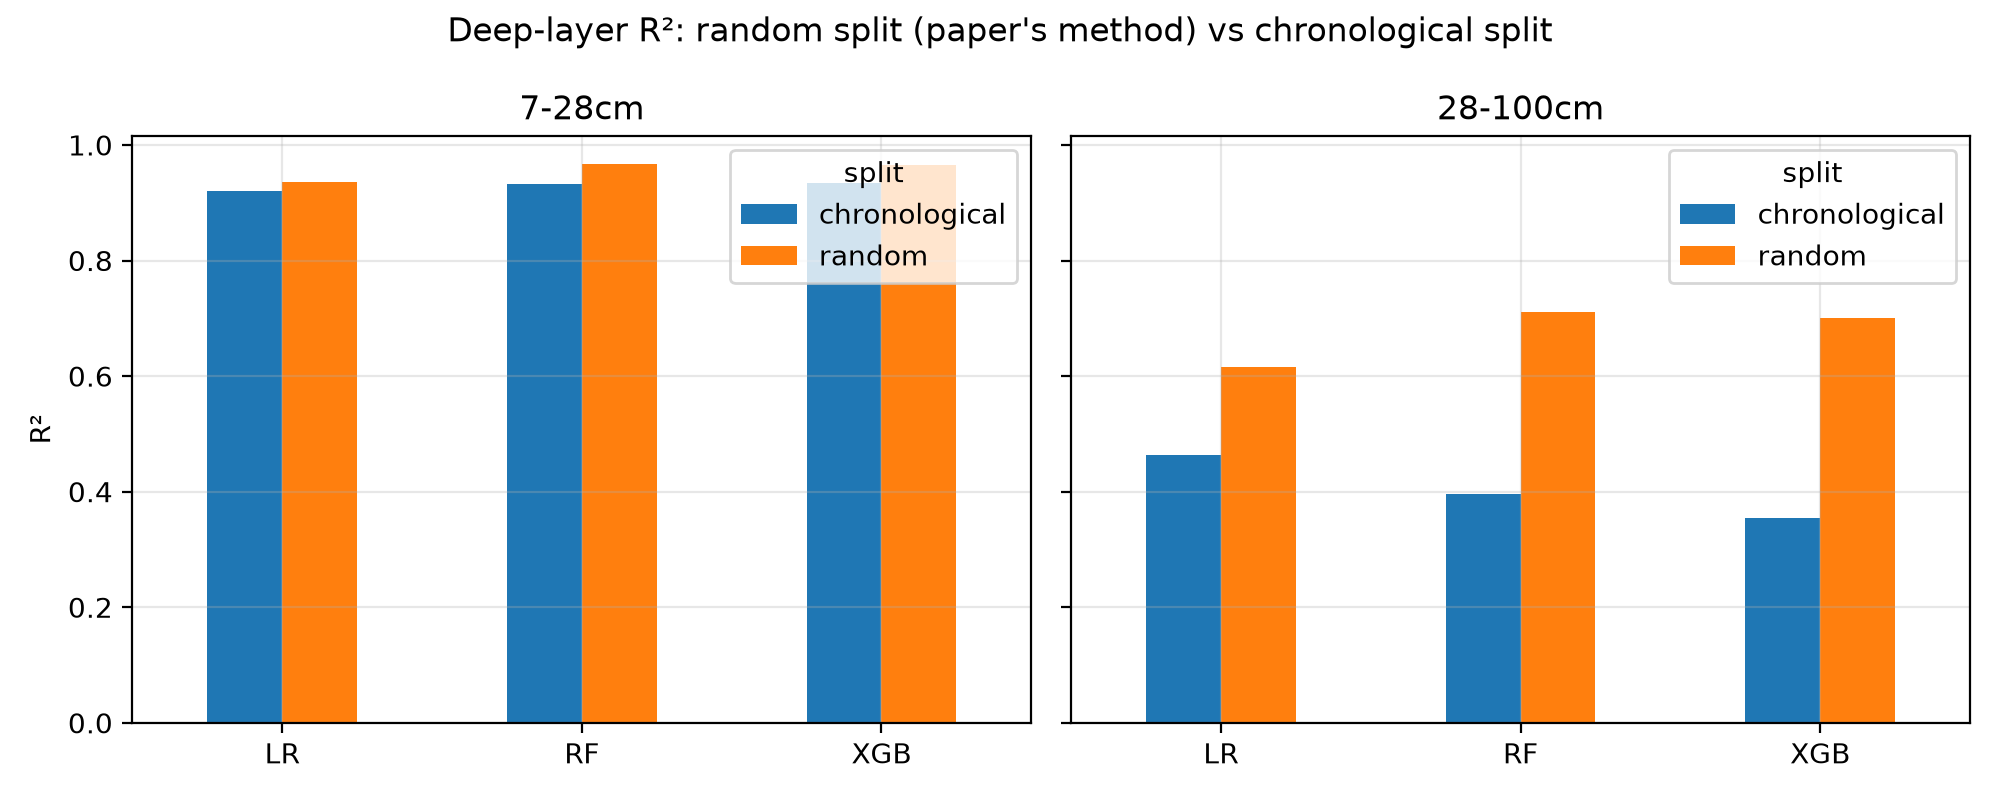
\includegraphics[width=0.95\textwidth]{figures/fig2_split_comparison.png}
\caption{Deep-layer $R^2$ under random vs.\ chronological train/test split. Random splitting inflates apparent performance, especially for the 28--100~cm layer where RF $R^2$ drops from 0.71 (random) to 0.40 (chronological).}
\label{fig:fig2}
\end{figure}

\begin{figure}[H]
\centering
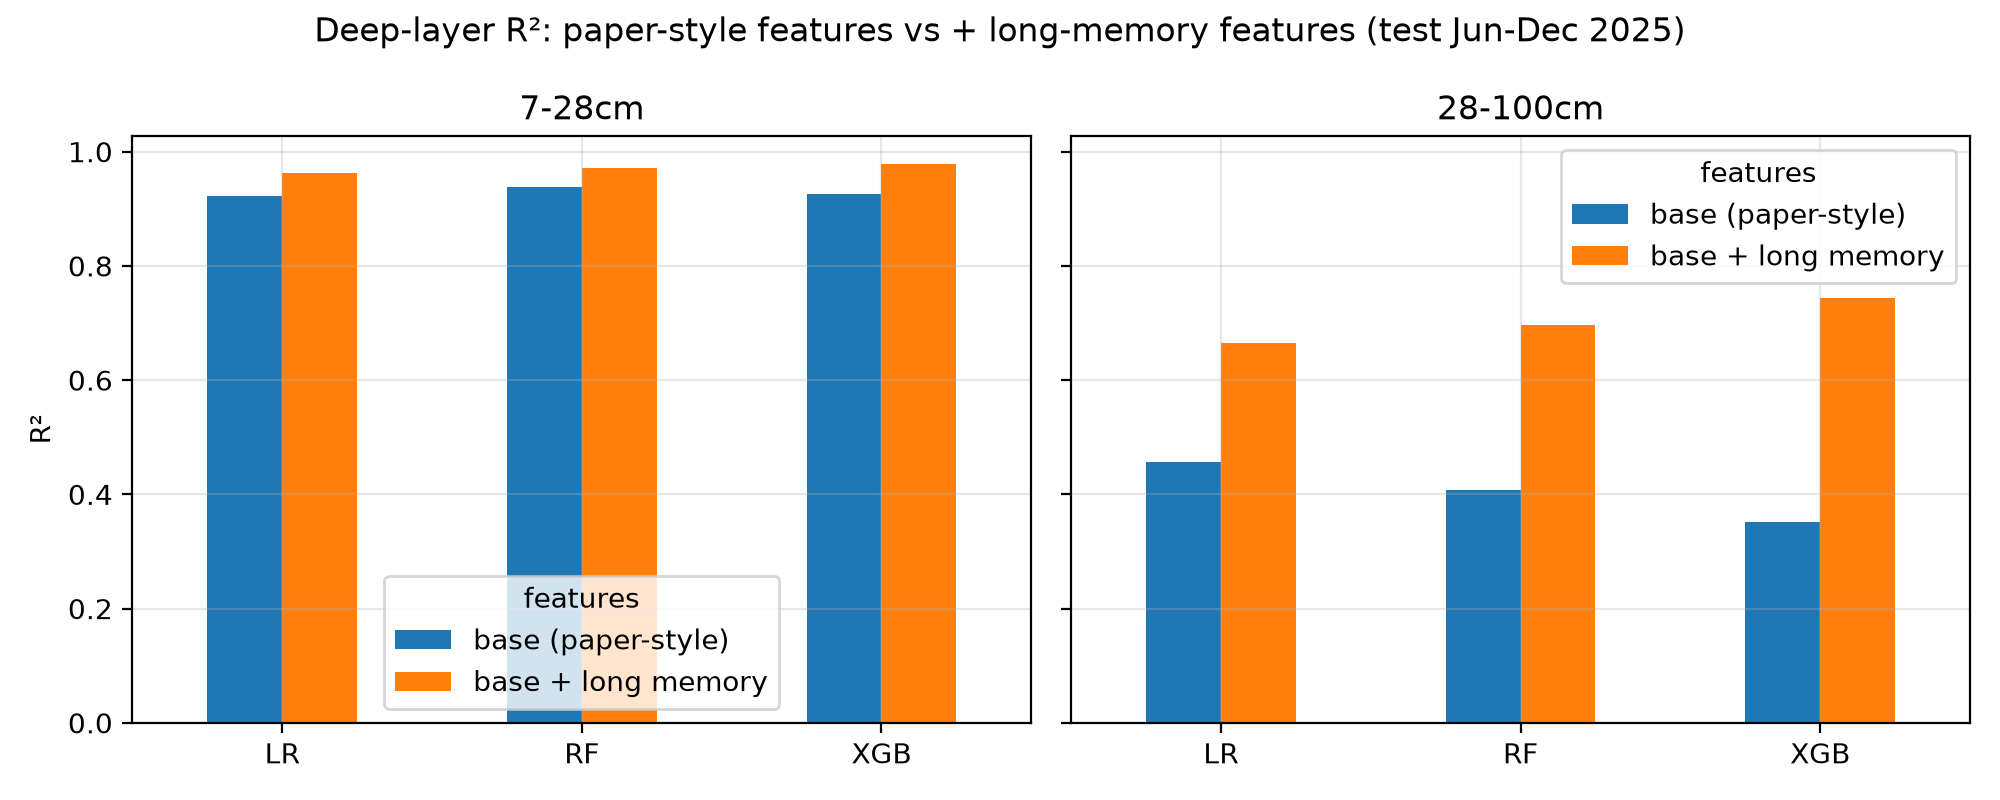
\includegraphics[width=0.95\textwidth]{figures/fig3_long_memory.png}
\caption{Effect of adding long-memory features (7--30-day rolling averages) to the deep-layer models. All three algorithms benefit substantially, with the largest gains for the 28--100~cm layer.}
\label{fig:fig3}
\end{figure}

\begin{figure}[H]
\centering
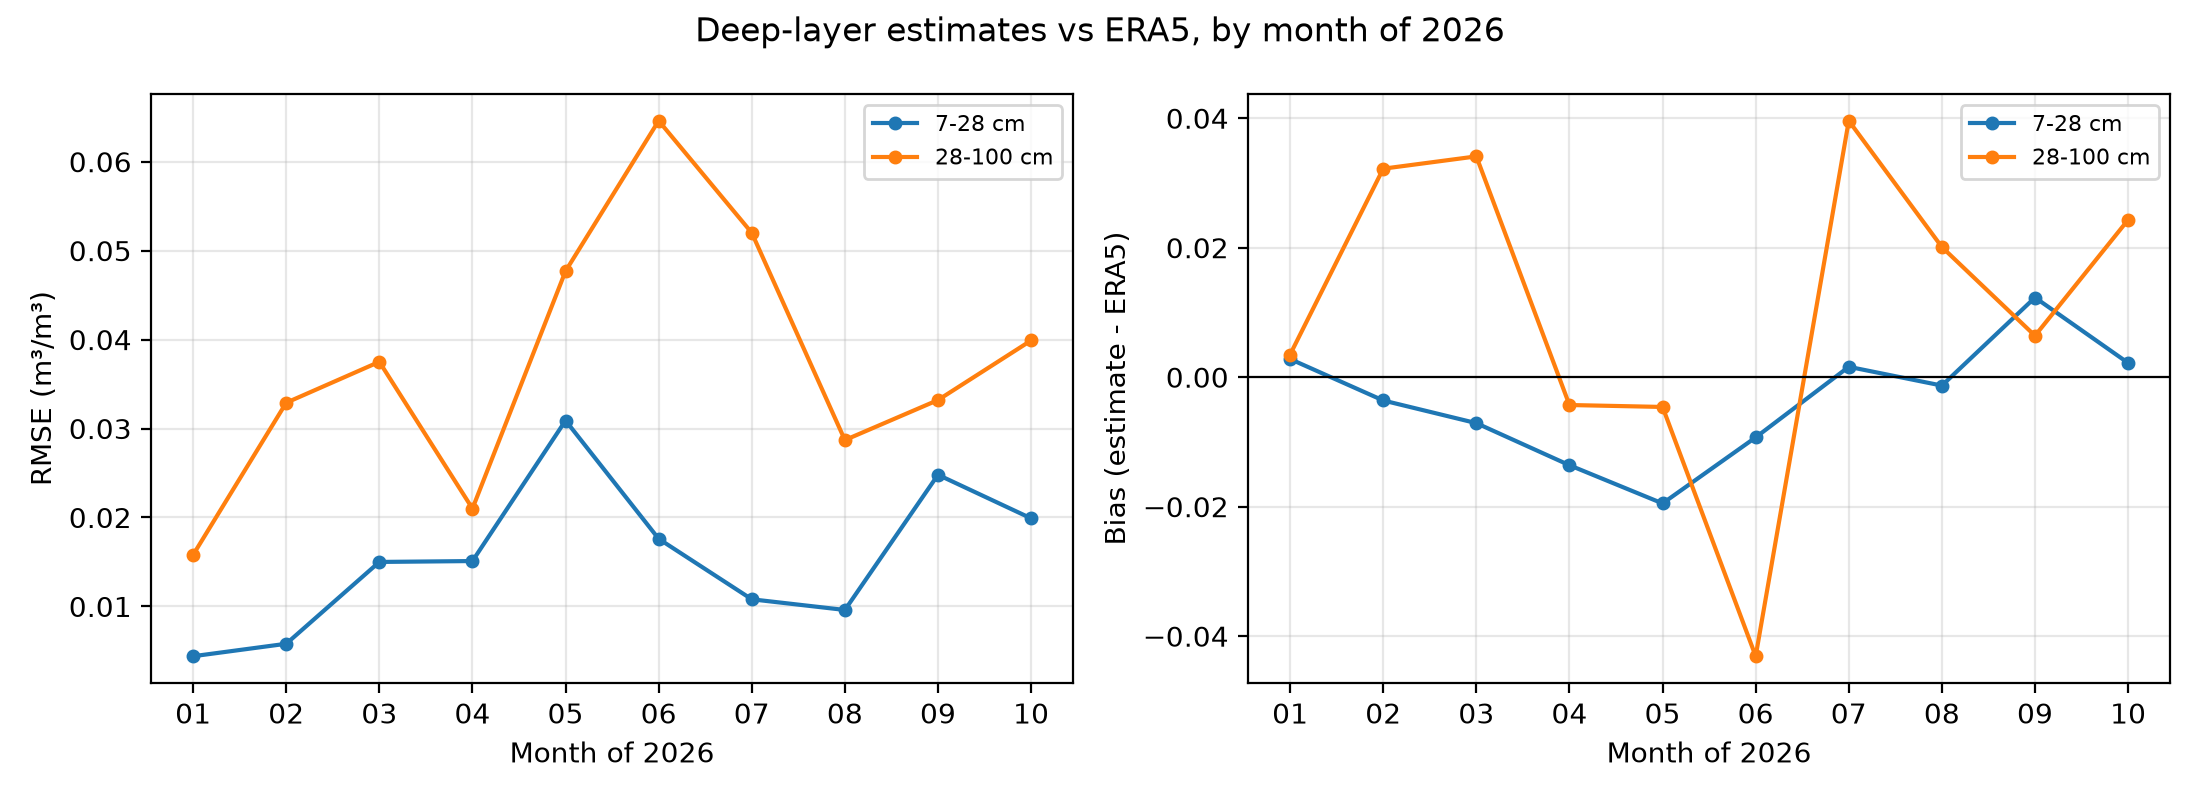
\includegraphics[width=0.95\textwidth]{figures/fig4_deep_2026_monthly.png}
\caption{Deep-layer estimation error by month of 2026. Left: RMSE. Right: Bias. The 7--28~cm model is stable across months; the 28--100~cm model shows higher RMSE in early 2026 and a persistent positive bias.}
\label{fig:fig4}
\end{figure}

\begin{figure}[H]
\centering
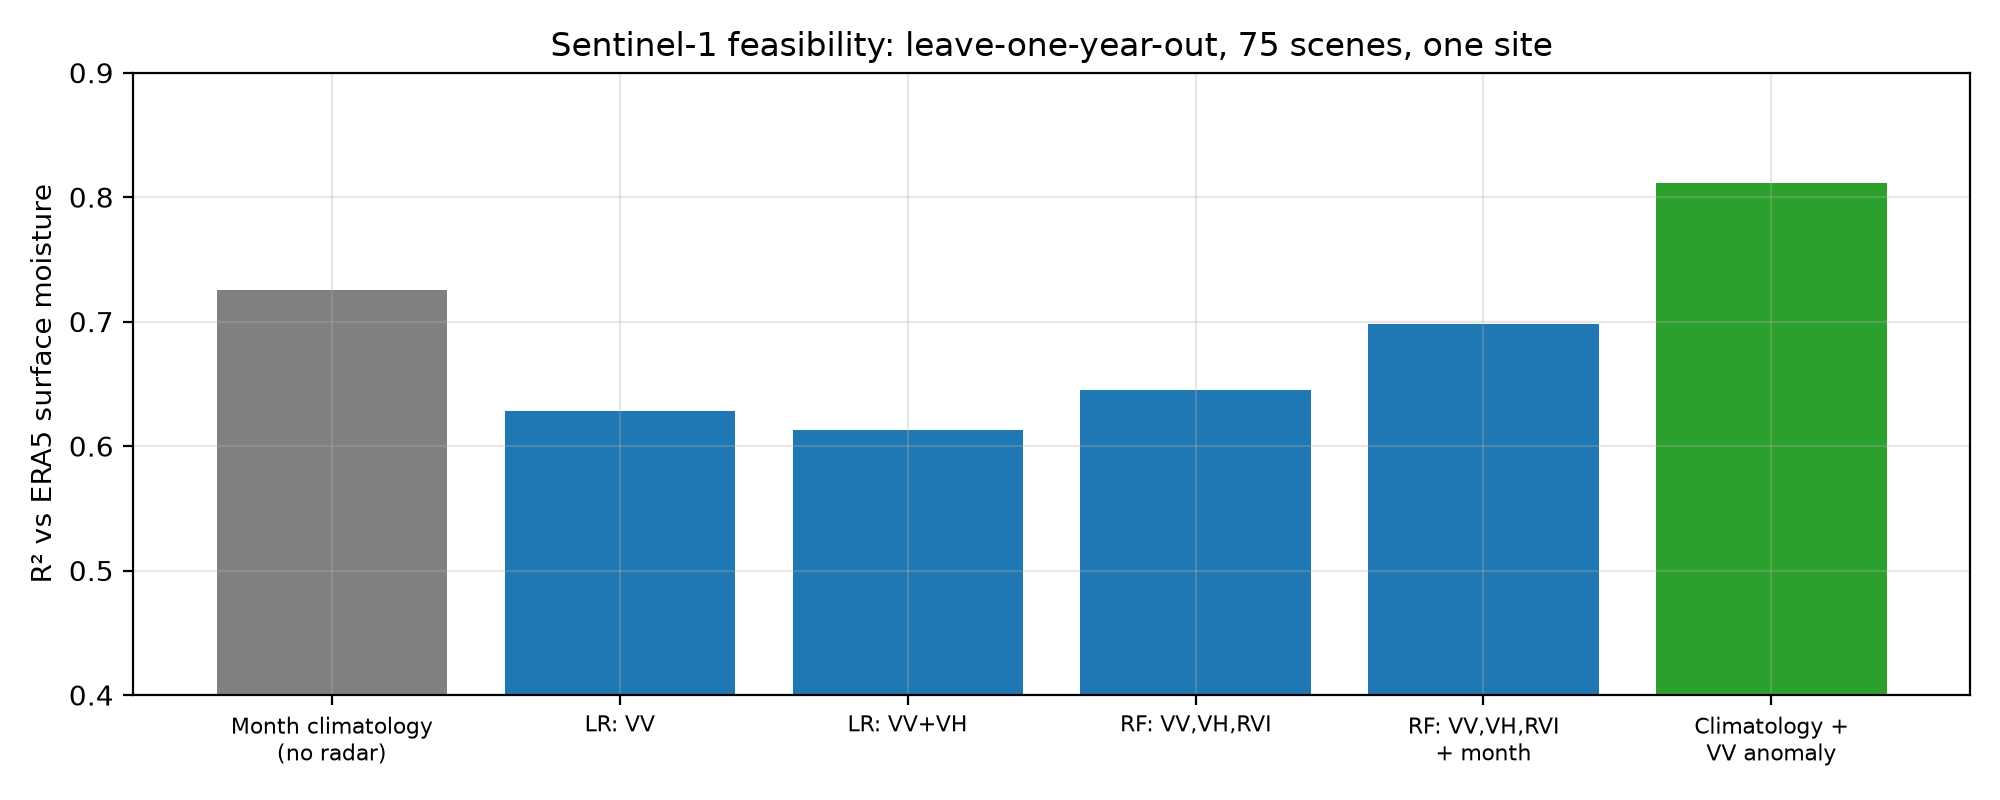
\includegraphics[width=0.95\textwidth]{figures/fig5_satellite_feasibility.png}
\caption{Sentinel-1 feasibility study results. Raw radar models (blue) underperform climatology (grey) due to vegetation confounding. The anomaly-based approach (green, rightmost) achieves $R^2 = 0.81$ by separating the seasonal cycle from genuine moisture variations.}
\label{fig:fig5}
\end{figure}

\begin{figure}[H]
\centering
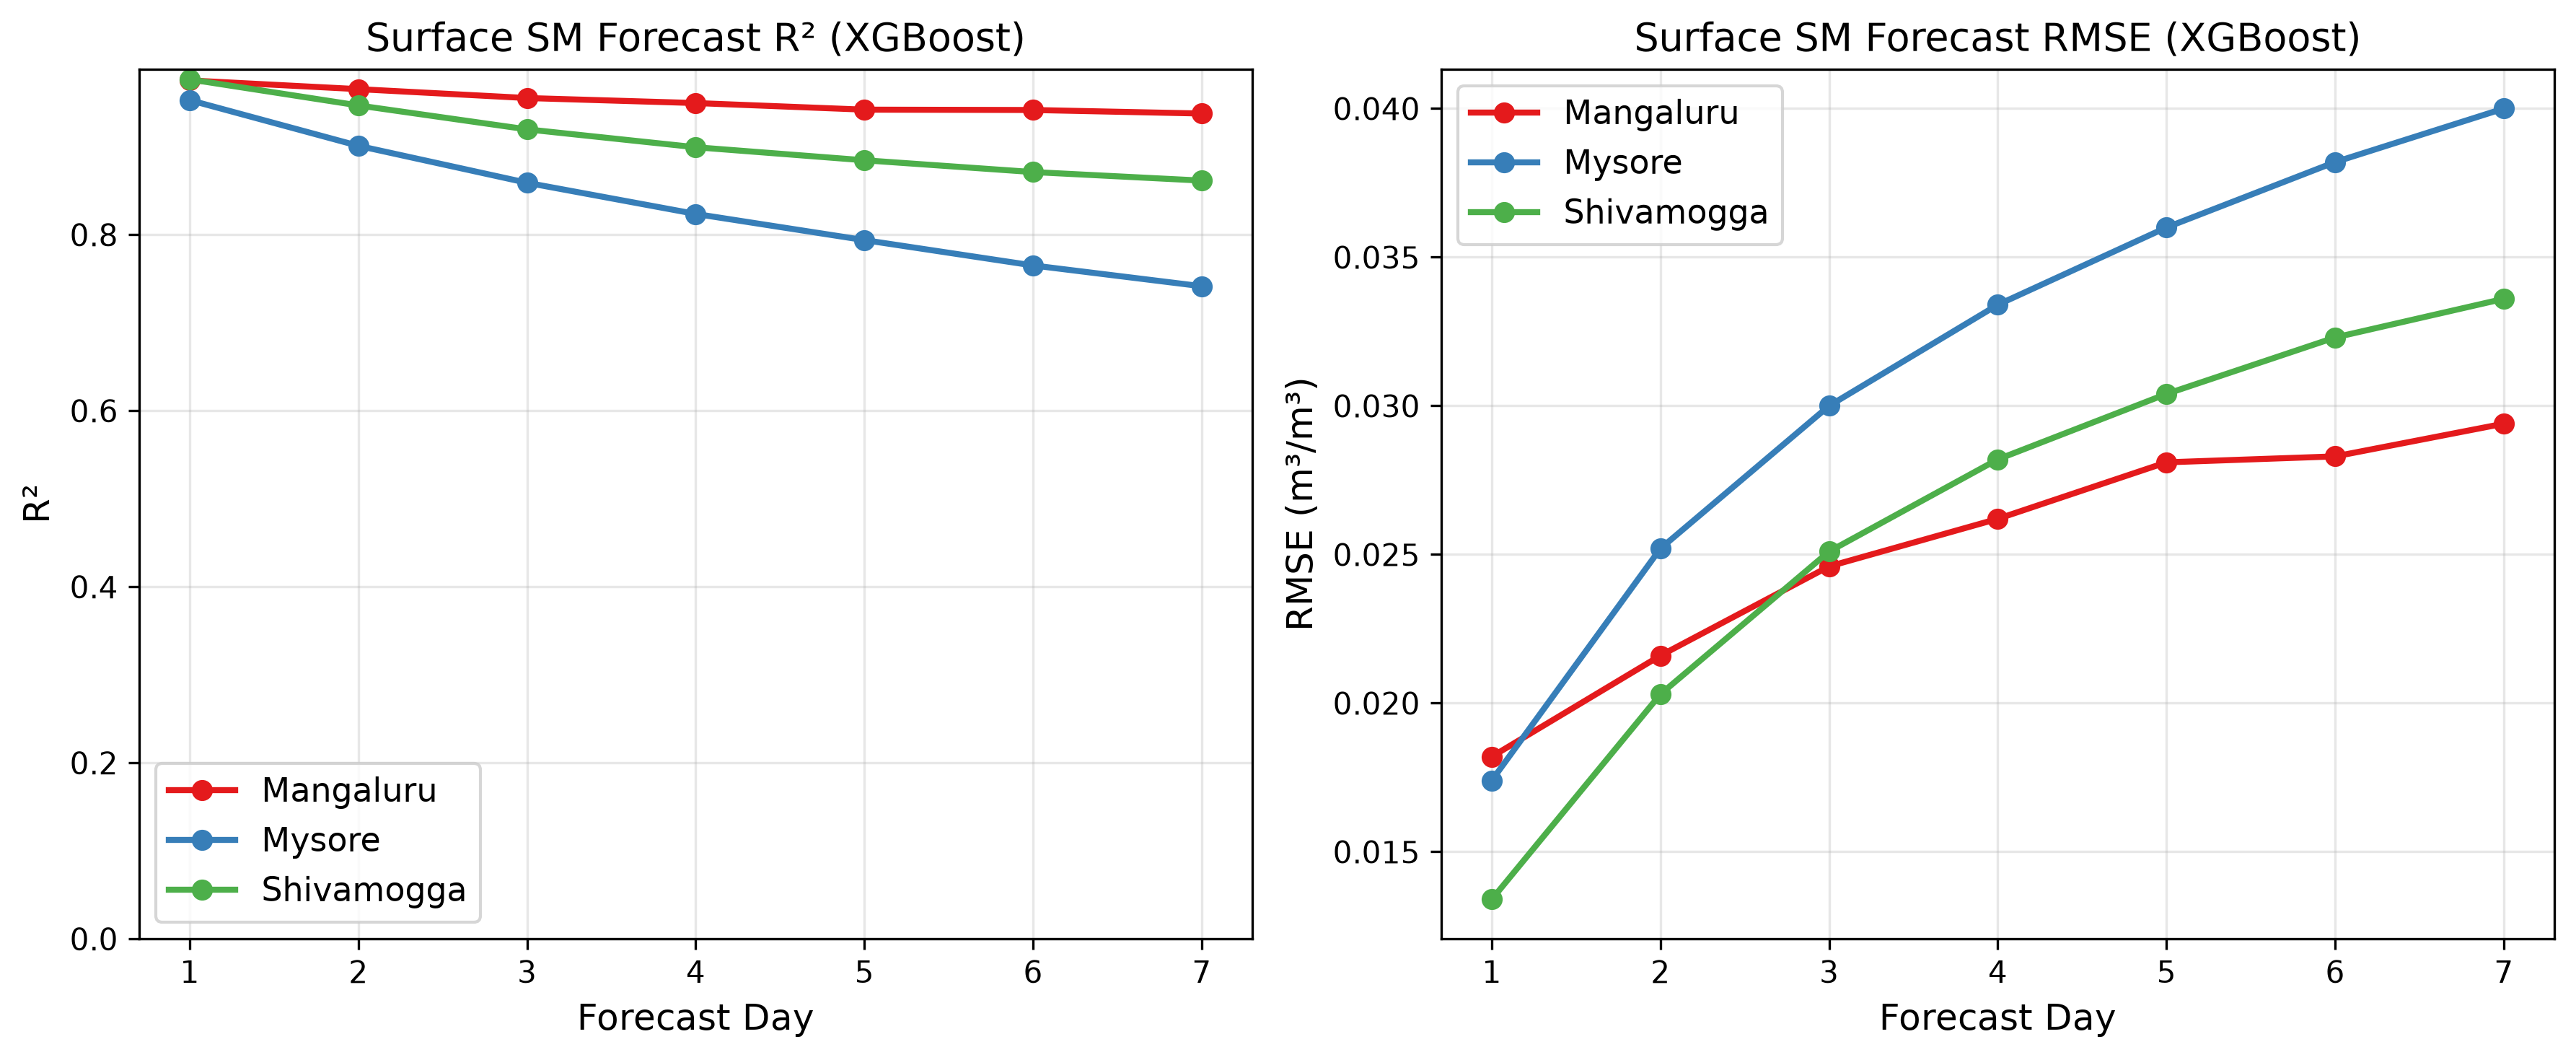
\includegraphics[width=0.95\textwidth]{figures/fig6_cross_site_forecast.png}
\caption{Cross-site surface soil moisture (0--7~cm) forecasting skill comparison across Mangaluru (red), Mysore (blue), and Shivamogga (green) over 1 to 7 lead days. Left: $R^2$. Right: RMSE (m$^3$/m$^3$).}
\label{fig:fig6_forecast}
\end{figure}

\begin{figure}[H]
\centering
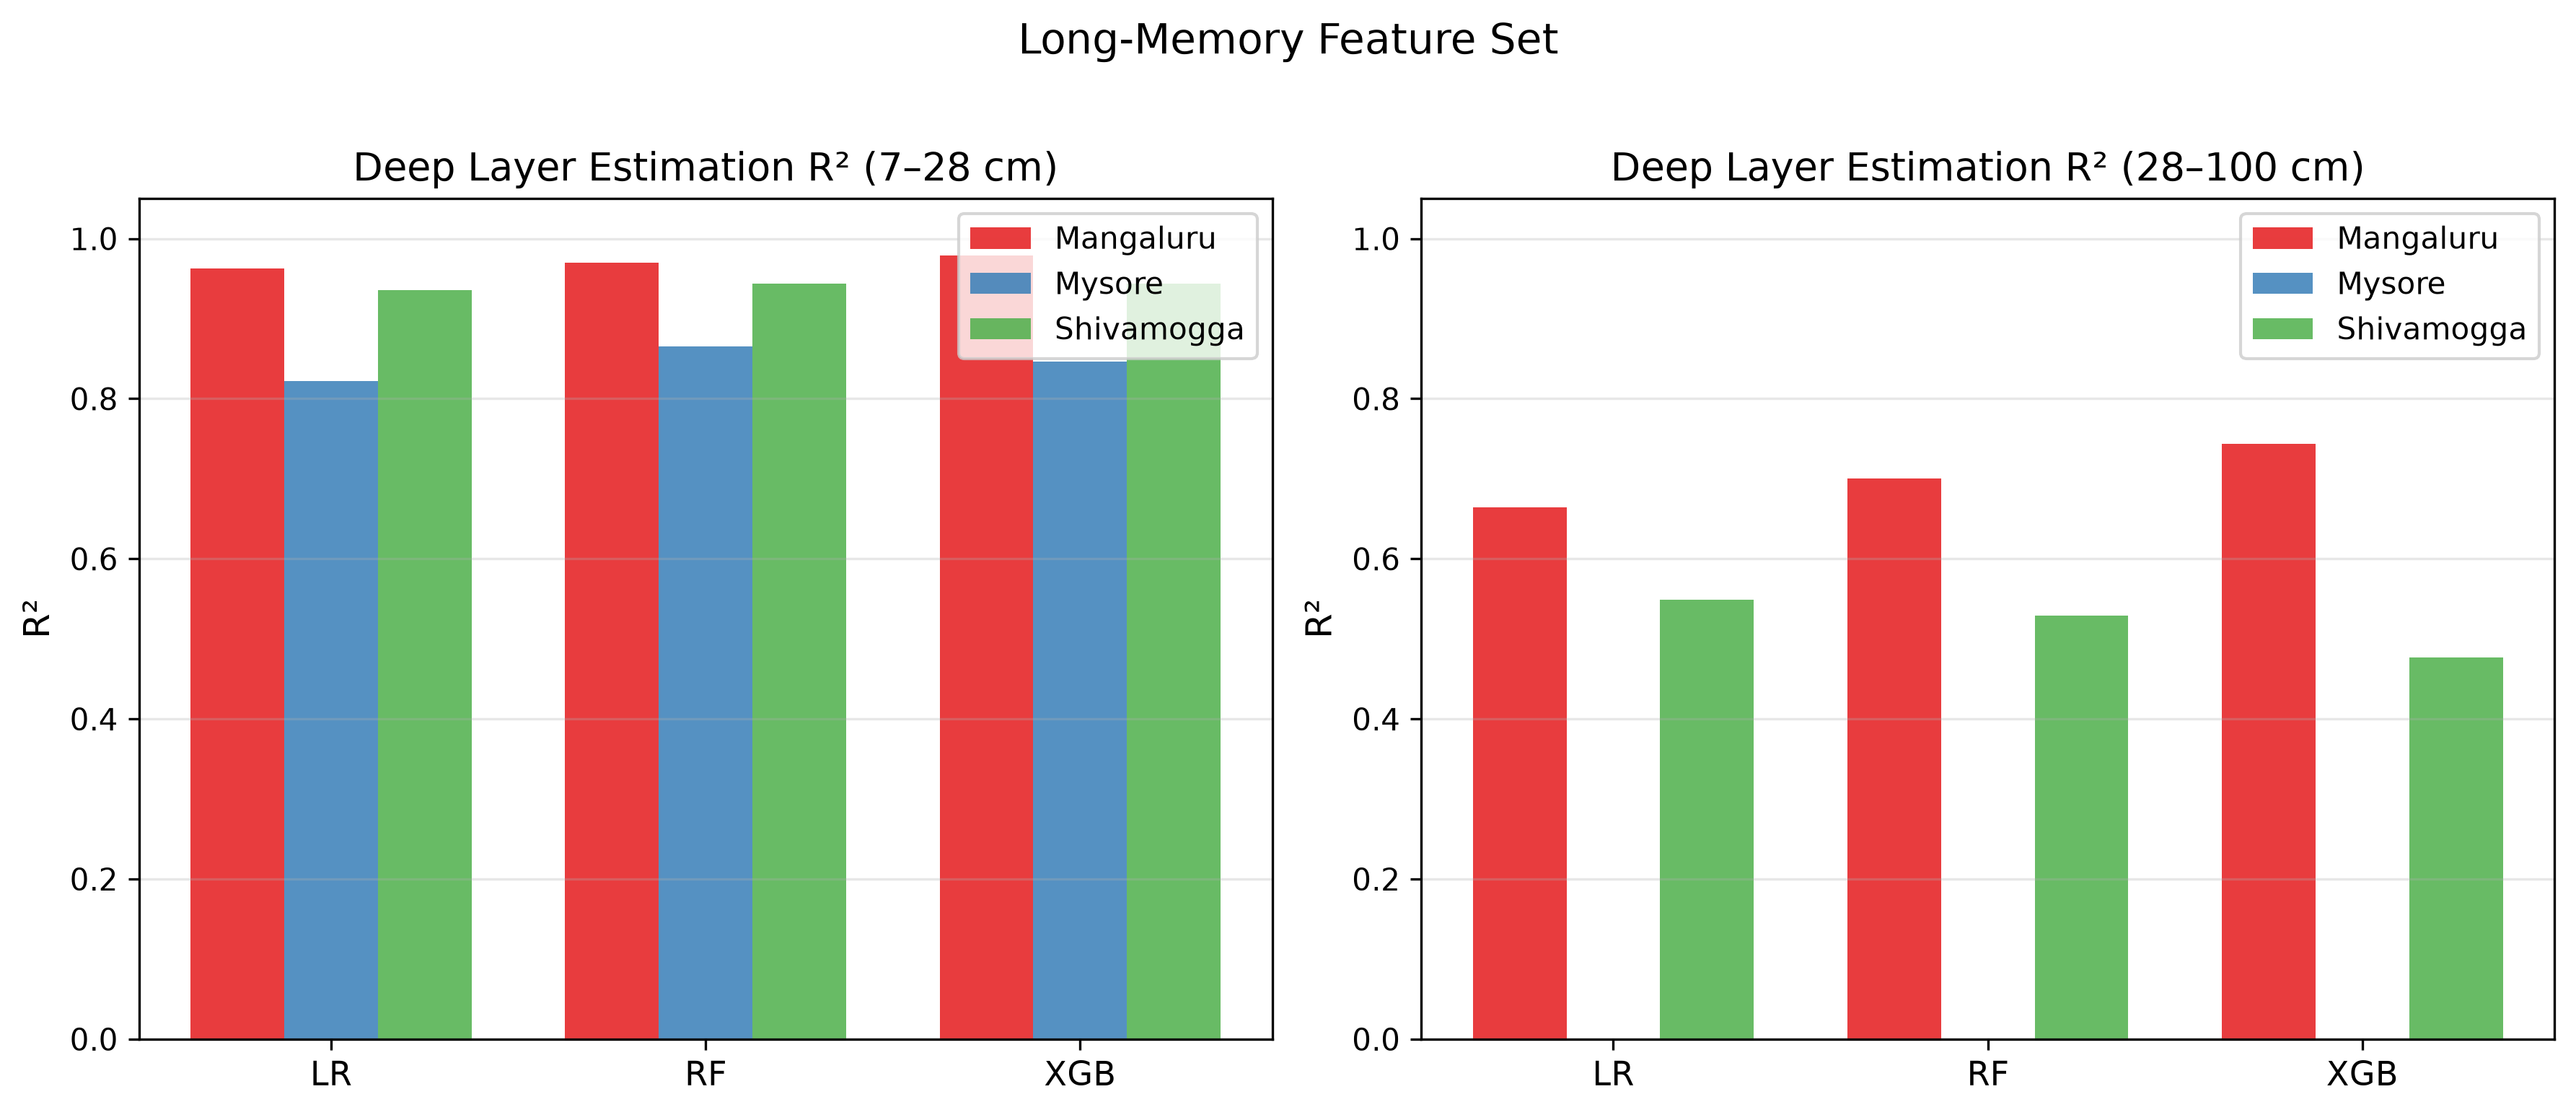
\includegraphics[width=0.95\textwidth]{figures/fig7_cross_site_deep.png}
\caption{Cross-site comparison of deep-layer estimation skill ($R^2$) with the long-memory feature set across all three machine learning algorithms (Linear Regression, Random Forest, and XGBoost). Left: Intermediate root-zone (7--28~cm). Right: Deep root-zone (28--100~cm).}
\label{fig:fig7_deep}
\end{figure}

\begin{figure}[H]
\centering
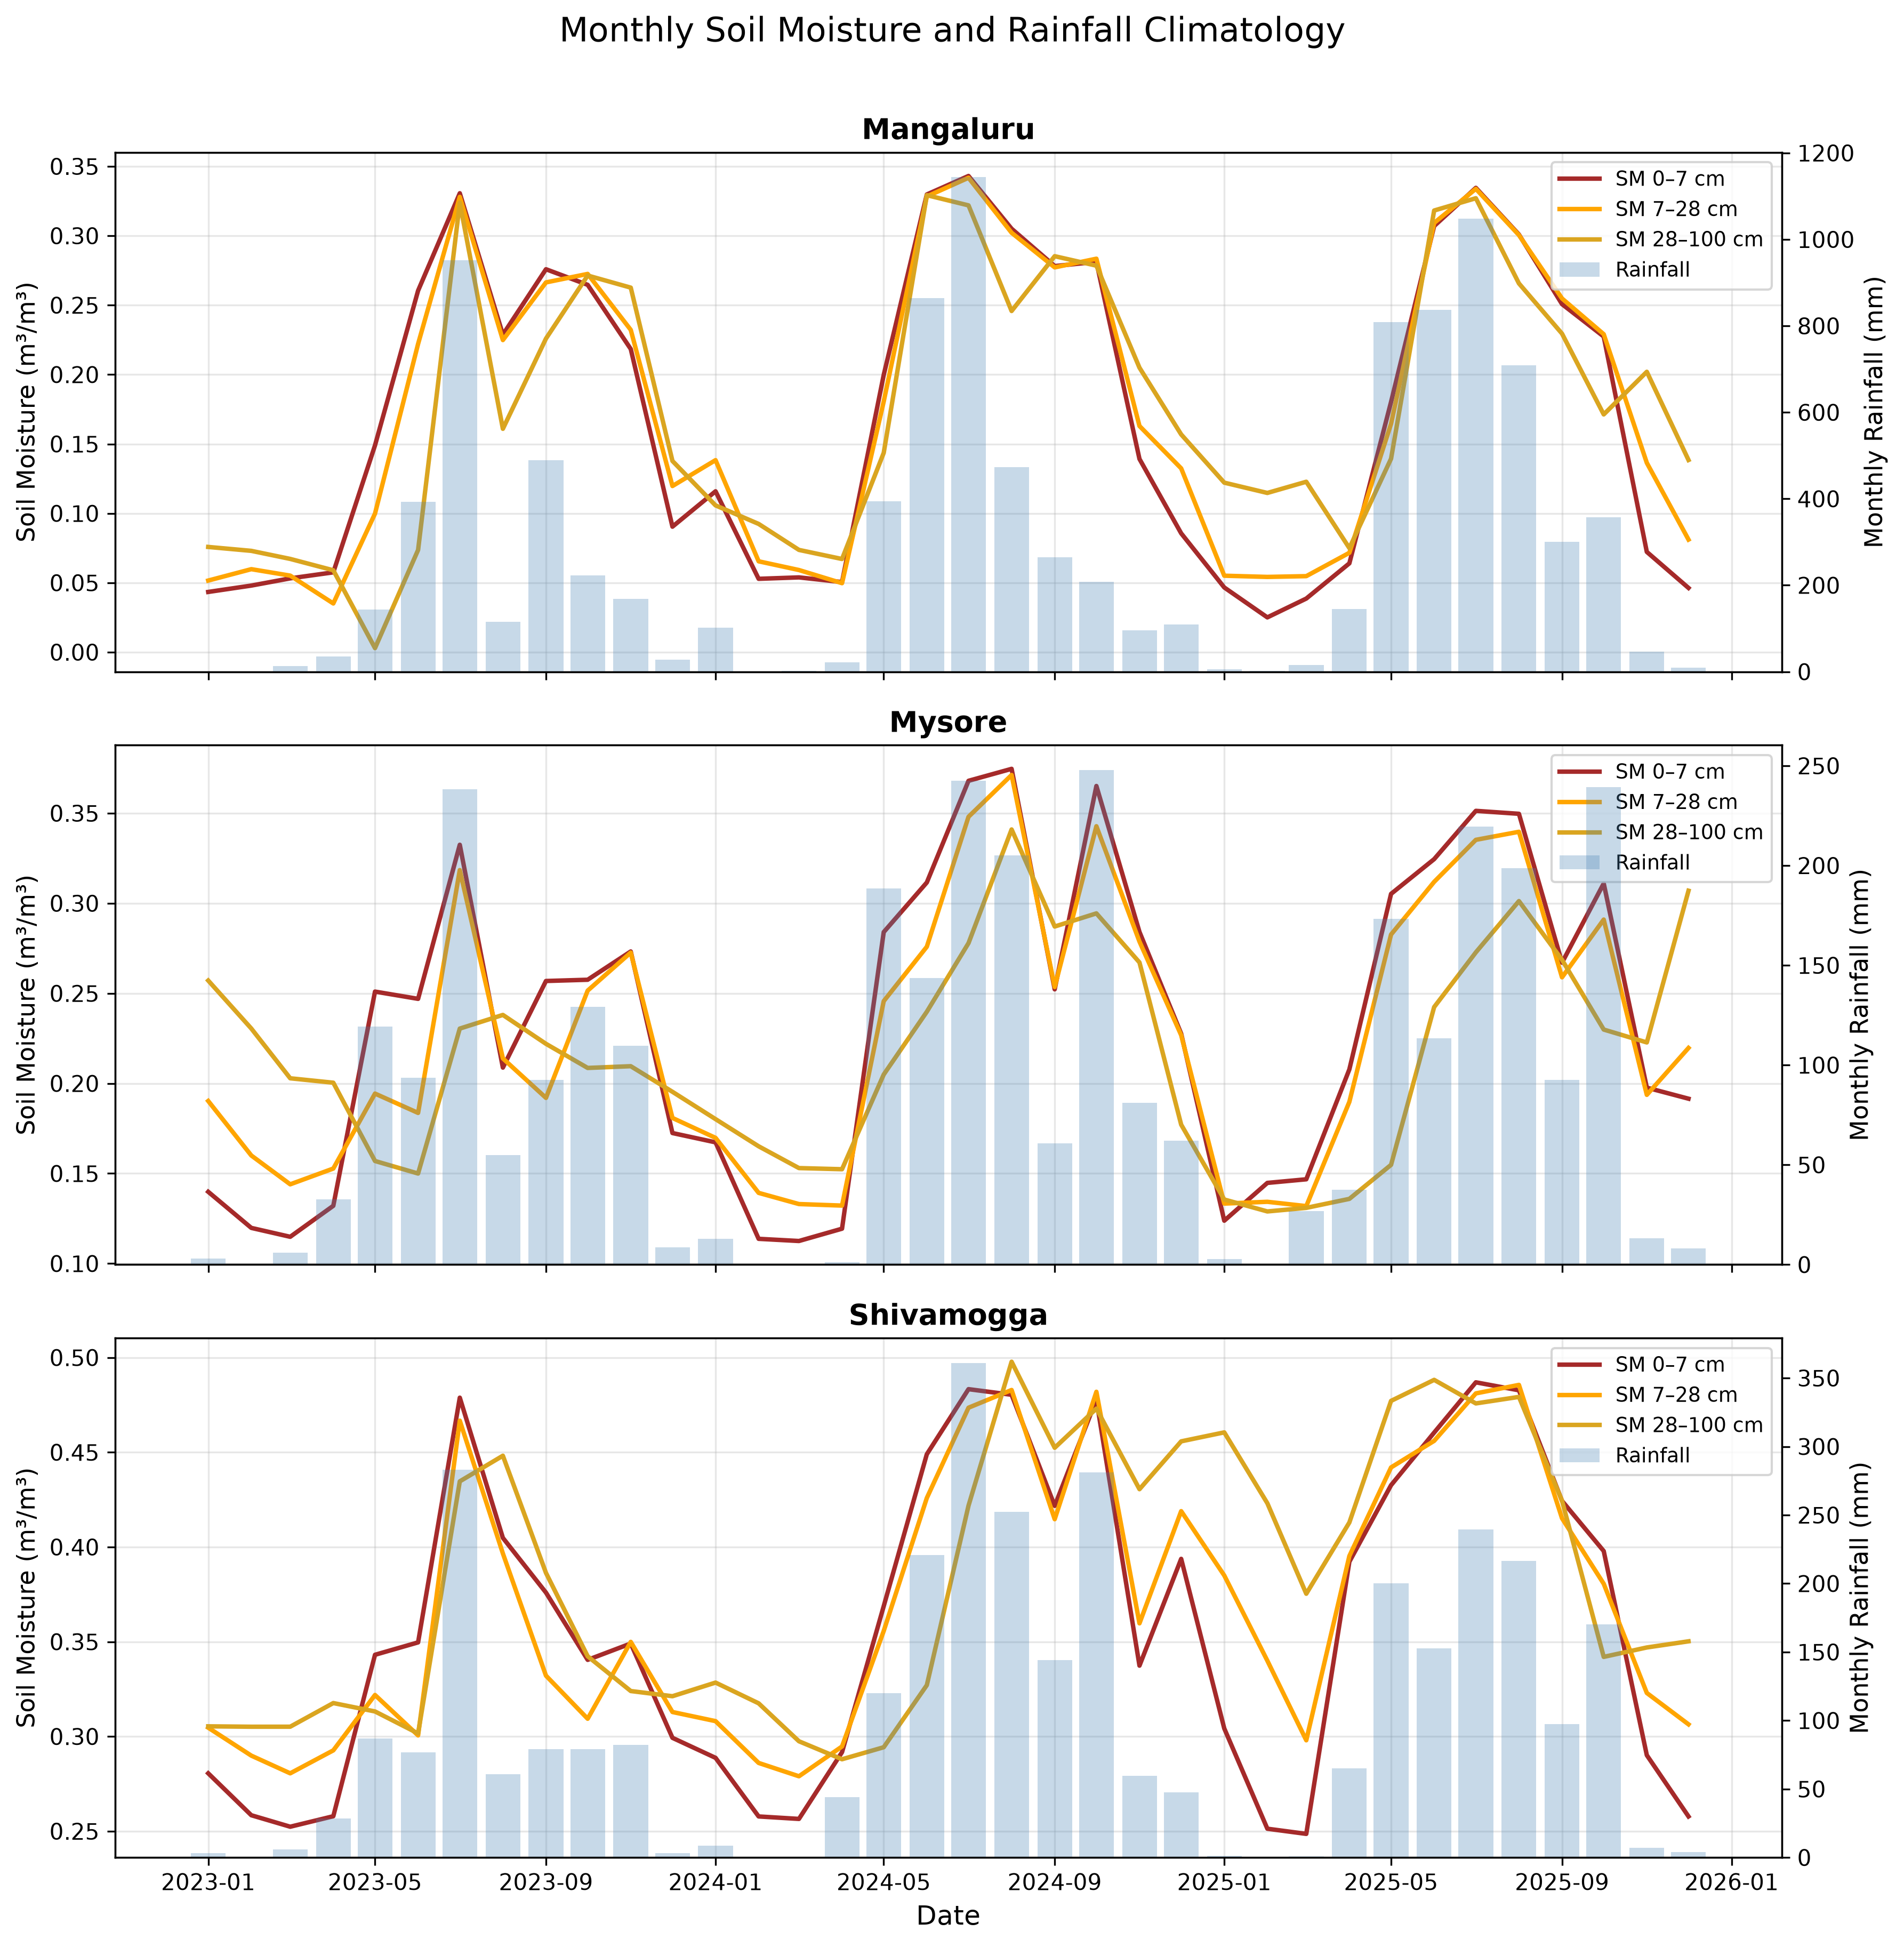
\includegraphics[width=0.95\textwidth]{figures/fig8_site_climatology.png}
\caption{Monthly mean soil moisture profiles across depths (0--7~cm, 7--28~cm, 28--100~cm) and total precipitation climatologies for Mangaluru, Mysore, and Shivamogga (2023--2025).}
\label{fig:fig8_climatology}
\end{figure}


% ══════════════════════════════════════════════════════════════════════
%  CHAPTER 9 — DISCUSSION
% ══════════════════════════════════════════════════════════════════════

\section{Discussion}

\subsection{Advances Over the Reference Paper}

\begin{enumerate}
    \item \textbf{Realistic weather inputs:} Training on archived ECMWF forecasts rather than ERA5 observations eliminates the train/test distribution mismatch that silently degrades the ERA5-trained model in operation. The $R^2$ improvement at day~7 (from 0.586 to 0.732) is substantial and practically meaningful.
    
    \item \textbf{Long-memory features:} The addition of rolling precipitation and moisture averages almost doubles the $R^2$ for the 28--100~cm layer. This reflects the well-known hydrological principle that deep percolation is a slow, cumulative process.
    
    \item \textbf{Honest evaluation:} The use of chronological splitting reveals that random-split results (as used in the reference paper) overstate deep-layer model performance by 25--50\% for the 28--100~cm layer.
    
    \item \textbf{Tropical site:} Applying the framework to Mangaluru --- a site with extreme monsoon seasonality --- tests the method's robustness beyond temperate or semi-arid conditions.

    \item \textbf{Multi-site cross-regional validation:} Extending the entire pipeline across three diverse agro-climatic zones in Karnataka (coastal Mangaluru, semi-arid plateau Mysore, and Ghats-transition Shivamogga) rigorously demonstrates that the recursive XGBoost forecaster maintains robust skill across contrasting hydrological regimes, dramatically outperforming persistence everywhere.
\end{enumerate}

\subsection{Limitations}

\begin{enumerate}
    \item \textbf{Deep-layer transferability in arid/plateau regimes:} While surface forecasting transferred robustly across all three climatic zones ($R^2 > 0.74$ at Day 7), deep-layer profile estimation at 28--100~cm in Mysore was constrained by negligible rainfall infiltration through the root barrier. In such leeward regimes, purely statistical models require coupling with local soil hydraulic parameters or baseflow drainage physics.
    
    \item \textbf{Reanalysis as ground truth:} ERA5-Land is a model product, not an in-situ measurement. Errors in ERA5-Land become errors in both our training targets and validation references.
    
    \item \textbf{28--100~cm estimation noise:} The deepest layer model has RMSE of $\sim$0.04~m\textsuperscript{3}/m\textsuperscript{3} on a signal that typically ranges between 0.05 and 0.12~m\textsuperscript{3}/m\textsuperscript{3}. This means daily fluctuations are unreliable; only the general moisture level is informative.
    
    \item \textbf{Error accumulation:} Recursive forecasting compounds errors. By day~7, the forecast RMSE is roughly 2.3$\times$ the day-1 RMSE.
    
    \item \textbf{Satellite module:} The Sentinel-1 feasibility study uses only $\sim$75 scenes at one point. It demonstrates potential but is far from an operational retrieval algorithm.
\end{enumerate}

\subsection{Future Work}

\begin{itemize}
    \item \textbf{In-situ sensor cross-validation}: Validate model predictions against physical dielectric sensor probes from Karnataka agricultural university research stations.
    \item \textbf{Deep learning architectures}: Explore hybrid LSTM-XGBoost or temporal convolutional networks to model asymmetrical drying curves across diverse soil textures.
    \item \textbf{Operational Sentinel-1 integration}: Assimilate SAR backscatter anomalies directly into the recursive forecaster to reset accumulated multi-day errors.
    \item \textbf{Irrigation scheduling support}: Couple volumetric root-zone forecasts with crop evapotranspiration ($ET_c$) models to provide actionable deficit-irrigation advisories for local farmers.
\end{itemize}

% ══════════════════════════════════════════════════════════════════════
%  CHAPTER 10 — CONCLUSION
% ══════════════════════════════════════════════════════════════════════

\section{Conclusion}

This project demonstrates that a machine-learning-based soil moisture forecasting and profiling system, adapted from Gao et al.\ (2026), can be successfully deployed and generalised across diverse tropical and subtropical agro-climatic zones in Karnataka, India:

\begin{itemize}
    \item \textbf{Surface forecasting}: An XGBoost model trained on real weather forecasts achieves $R^2 = 0.95$--$0.98$ at 1-day lead and $R^2 = 0.74$--$0.94$ at 7-day lead across Mangaluru, Mysore, and Shivamogga, consistently outperforming both persistence and oracle-weather-trained alternatives.
    
    \item \textbf{Cross-regional robustness}: In semi-arid regions such as Mysore, where persistence collapses to $R^2 = 0.22$ by Day 7 due to convective volatility, the XGBoost model sustains $R^2 = 0.74$, demonstrating high utility for water resource planning.

    \item \textbf{Deep-layer profiling}: Progressive chaining with long-memory features yields $R^2 = 0.87$--$0.98$ for the intermediate root-zone (7--28~cm) and up to $R^2 = 0.74$ for the 28--100~cm layer in high-precipitation zones --- eliminating the need for expensive subsurface sensor infrastructure.
    
    \item \textbf{Satellite feasibility}: An anomaly-based Sentinel-1 approach achieves $R^2 = 0.81$ for surface moisture, demonstrating that free satellite radar data can provide independent observational constraints.
    
    \item \textbf{Operational readiness}: An enhanced live Streamlit dashboard brings these models together for all three study regions, providing interactive geospatial visualisation, latency-gap bridging, and uncertainty-aware forecasts.
\end{itemize}

The key methodological takeaway is the importance of \textit{training under realistic conditions}: using real weather forecasts instead of perfect reanalysis data, using chronological instead of random data splits, and including physically motivated features (long-memory rolling averages) that match the timescales of the target process.

% ══════════════════════════════════════════════════════════════════════
%  REFERENCES
% ══════════════════════════════════════════════════════════════════════

\section*{References}
\addcontentsline{toc}{section}{References}

\begin{enumerate}[label={[\arabic*]}]
    \item Gao, Y., et al.\ (2026). Soil moisture forecasting with machine learning: a recursive multi-step approach using weather forecast inputs. \textit{Smart Agricultural Technology}. \url{https://www.sciencedirect.com/science/article/pii/S2772375526006246}

    \item Chen, T.\ and Guestrin, C.\ (2016). XGBoost: A Scalable Tree Boosting System. \textit{Proceedings of the 22nd ACM SIGKDD International Conference on Knowledge Discovery and Data Mining}, pp.\ 785--794.

    \item Muñoz-Sabater, J., et al.\ (2021). ERA5-Land: A state-of-the-art global reanalysis dataset for land applications. \textit{Earth System Science Data}, 13(9), pp.\ 4349--4383.

    \item Torres, R., et al.\ (2012). GMES Sentinel-1 mission. \textit{Remote Sensing of Environment}, 120, pp.\ 9--24.

    \item Zink, M., et al.\ (2015). The Global Soil Moisture Patterns Observed by SMAP, SMOS and ERA-Interim. \textit{Geophysical Research Letters}, 42(20).

    \item Open-Meteo.\ (2024). Free Weather API. \url{https://open-meteo.com/}

    \item Gorelick, N., et al.\ (2017). Google Earth Engine: Planetary-scale geospatial analysis for everyone. \textit{Remote Sensing of Environment}, 202, pp.\ 18--27.

    \item Pedregosa, F., et al.\ (2011). Scikit-learn: Machine Learning in Python. \textit{Journal of Machine Learning Research}, 12, pp.\ 2825--2830.
    
    \item Wang, D., Xu, S., Zhang, C., Chen, M., et al.\ (2026). Estimation of multi-layer soil moisture in agricultural irrigation areas based on a feature-level integrated LSTM-XGBoost model. \textit{Agricultural Water Management}.
\end{enumerate}

\end{document}
